\chapter{Bipolar-valued undirected graphs}
\label{sec:21}

\abstract*{ The chapter introduces bipolar-valued undirected graphs and illustrates several special graph models and algorithms like Q-coloring, MIS and clique enumeration, line graphs and maximal matchings, grid graphs, and $n$-cycle graphs and their non-isomorphic maximal independent sets of vertices.}

\abstract{ The chapter introduces bipolar-valued undirected graphs and illustrates several special graph models and algorithms like Q-coloring, MIS and clique enumeration, line graphs and maximal matchings, grid graphs, and $n$-cycle graphs with their non-isomorphic maximal independent sets of vertices.}

% \paragraph{Introduction}

% \noindent The \Digraph resoureces provide the \texttt{graphs} module module\index{graphs@\texttt{graphs} module} with the following graph models:
% \begin{figure}[h]
% %\sidecaption[t]
% 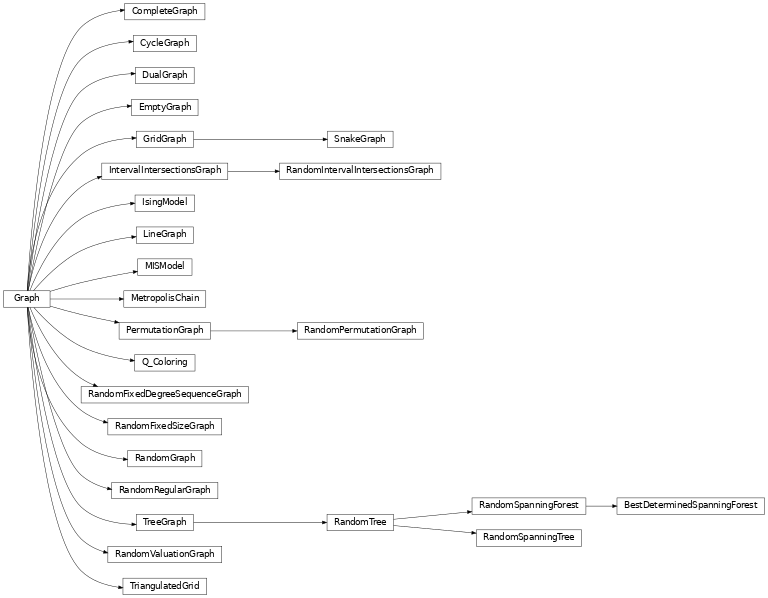
\includegraphics[width=11cm]{Figures/21-0-graphsInheritance.png}
% \caption{Inheritance digram of the \texttt{graphs} module} 
% \label{fig:21.0}       % Give a unique label
% \end{figure}


\section{Implementing simple graphs}
\label{sec:21.1}

In the \Digraph \texttt{graphs} module\index{graphs@\texttt{graphs} module}, the root \texttt{Graph} class \index{Graph@\texttt{Graph} class} provides a generic simple graph model, without loops and multiple links. A given object of this \texttt{Graph} type contains at least the following attributes:
\begin{enumerate}[topsep=1pt]
\item \texttt{name}: usually the name of the stored instance.
\item \texttt{vertices}: a dictionary with \texttt{name} and \texttt{shortName} attributes,
\item \texttt{order}: the number of vertices,
\item \texttt{valuationDomain}: a dictionary with three entries: the minimum ($-1$, means certainly no link), the median ($0$, means missing information) and the maximum characteristic value ($+1$, means certainly a link),
\item \texttt{edges} : a dictionary with \emph{frozensets} \footnote{\href{https://docs.python.org/3.9/library/stdtypes.html?highlight=frozenset\#frozenset}{Python documentation}} of pairs of vertices as keys carrying a characteristic value in the range of the previous valuation domain,
\item \texttt{size}: the number of positive edges,
\item \texttt{gamma}: a dictionary containing the direct neighbors of each vertex, automatically added by the object constructor.
\end{enumerate}

\paragraph{\textbf{Example Python terminal session}}

\noindent A random crisp graph instance can be generated with the \texttt{RandomGraph} class (see Lines 1-2 in Listing~\vref{list:21.1} below).\index{RandomGraph@\texttt{RandomGraph} class} 
\begin{lstlisting}[caption={Generating a randm graph instance},label=list:21.1]
>>> from graphs import RandomGraph
>>> g = RandomGraph(order=7,edgeProbability=0.5)
>>> g.save(fileName='tutorialGraph')
\end{lstlisting}

The saved \texttt{Graph} instance, named \texttt{tutorialGraph.py}, is encoded as shown in Listing~\vref{list:21.2}.
\begin{lstlisting}[caption={Stored instance of a random graph},label=list:21.2]
  # Graph instance saved in Python format
   from decimal import Decimal
   vertices = {
    'v1': {'shortName': 'v1', 'name': 'random vertex'},
    'v2': {'shortName': 'v2', 'name': 'random vertex'},
    'v3': {'shortName': 'v3', 'name': 'random vertex'},
    'v4': {'shortName': 'v4', 'name': 'random vertex'},
    'v5': {'shortName': 'v5', 'name': 'random vertex'},
    'v6': {'shortName': 'v6', 'name': 'random vertex'},
    'v7': {'shortName': 'v7', 'name': 'random vertex'},
   }
   valuationDomain = {
     'min':Decimal('-1'),'med':Decimal('0'),
     'max':Decimal('1')}
   edges = {
    frozenset(['v1','v2']) : Decimal('-1'), 
    frozenset(['v1','v3']) : Decimal('-1'), 
    frozenset(['v1','v4']) : Decimal('-1'), 
    frozenset(['v1','v5']) : Decimal('1'), 
    frozenset(['v1','v6']) : Decimal('-1'), 
    frozenset(['v1','v7']) : Decimal('-1'), 
    frozenset(['v2','v3']) : Decimal('1'), 
    frozenset(['v2','v4']) : Decimal('1'), 
    frozenset(['v2','v5']) : Decimal('-1'), 
    frozenset(['v2','v6']) : Decimal('1'), 
    frozenset(['v2','v7']) : Decimal('-1'), 
    frozenset(['v3','v4']) : Decimal('-1'), 
    frozenset(['v3','v5']) : Decimal('-1'), 
    frozenset(['v3','v6']) : Decimal('-1'), 
    frozenset(['v3','v7']) : Decimal('-1'), 
    frozenset(['v4','v5']) : Decimal('1'), 
    frozenset(['v4','v6']) : Decimal('-1'), 
    frozenset(['v4','v7']) : Decimal('1'), 
    frozenset(['v5','v6']) : Decimal('1'), 
    frozenset(['v5','v7']) : Decimal('-1'), 
    frozenset(['v6','v7']) : Decimal('-1'), 
    }
\end{lstlisting}

The stored graph instance may be reloaded and plotted with the \texttt{export\-GraphViz()} method (see Fig.~\vref{fig:21.1}):
\begin{lstlisting}
>>> g = Graph('tutorialGraph')
>>> g.exportGraphViz()
  *---- exporting a dot file for GraphViz tools ---------*
   Exporting to tutorialGraph.dot
   fdp -Tpng tutorialGraph.dot -o tutorialGraph.png
\end{lstlisting}
\begin{figure}[h]
\sidecaption[t]
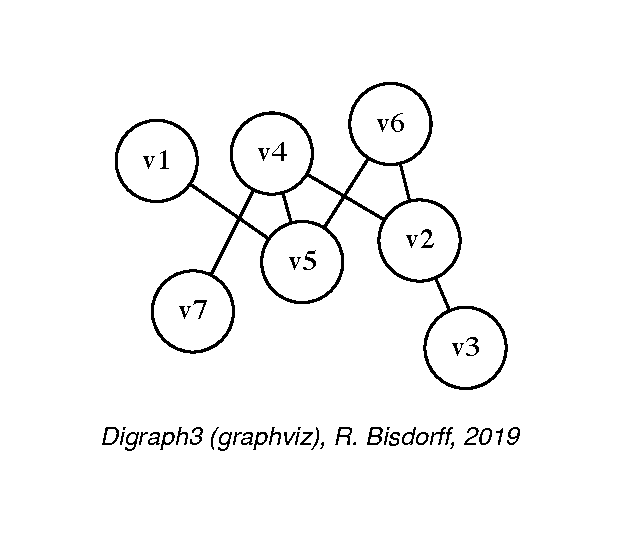
\includegraphics[width=7cm]{Figures/21-1-tutorialGraph.pdf}
\caption{Example simple graph instance} 
\label{fig:21.1}       % Give a unique label
\end{figure}

Properties, like the gamma function --the cover relation--, vertex degrees and neighbourhood depths are shown with a \texttt{showShort()} method. \index{showShort@\texttt{showShort()}}
\begin{lstlisting}[caption={Inspecting a graph instance},label=list:21.3]
>>> g.showShort()
  *---- short description of the graph ----*
   Name : 'tutorialGraph'
   Vertices :  ['v1','v2','v3','v4','v5','v6','v7']
   Valuation domain : {'min': -1, 'med': 0, 'max': 1}
   Gamma function   : 
    v1 -> ['v5']
    v2 -> ['v6', 'v4', 'v3']
    v3 -> ['v2']
    v4 -> ['v5', 'v2', 'v7']
    v5 -> ['v1', 'v6', 'v4']
    v6 -> ['v2', 'v5']
    v7 -> ['v4']
   degrees      :  [0, 1, 2, 3, 4, 5, 6]
   distribution :  [0, 3, 1, 3, 0, 0, 0]
   nbh depths   :  [0, 1, 2, 3, 4, 5, 6, 'inf.']
   distribution :  [0, 0, 1, 4, 2, 0, 0, 0]
\end{lstlisting}

A \texttt{Graph} instance corresponds bijectively to a symmetric \texttt{Digraph} instance and we can convert from one to the other with the \texttt{graph2Digraph()}\index{graph2Digraph@\texttt{graph2Digraph()}}, and vice versa, with the \texttt{digraph2Graph()} method (see Listing~\vref{list:21.4}).\index{digraph2Graph@\texttt{digraph2Graph()}} Thus, all computing resources of the \texttt{Digraph} class suitable for symmetric digraphs become readily available, and vice versa.
\begin{lstlisting}[caption={Conversion between graphs and digraphs},label=list:21.4]
>>> dg = g.graph2Digraph()
>>> dg.showRelationTable(ndigits=0,ReflexiveTerms=False)
  * ---- Relation Table -----
    S  |  'v1'  'v2'  'v3'  'v4'  'v5'  'v6'  'v7'	  
  -----|------------------------------------------
  'v1' |    -    -1    -1    -1     1    -1    -1	 
  'v2' |   -1     -     1     1    -1     1    -1	 
  'v3' |   -1     1     -    -1    -1    -1    -1	 
  'v4' |   -1     1    -1     -     1    -1     1	 
  'v5' |    1    -1    -1     1     -     1    -1	 
  'v6' |   -1     1    -1    -1     1     -    -1	 
  'v7' |   -1    -1    -1     1    -1    -1     -
>>> g1 = dg.digraph2Graph()
>>> g1
  *------- Digraph instance description ------*
   Instance class      : Digraph
   Instance name       : tutorialGraph
   Digraph Order       : 7
   Digraph Size        : 14
   Valuation domain    : [-1.00;1.00]
   Determinateness (%) : 100.00
   Attributes          : ['name', 'order', 'actions',
                          'valuationdomain', 'relation',
                          'gamma', 'notGamma']
\end{lstlisting}

\section{Q-coloring of a graph}
\label{25.2}

With the \texttt{Q\_Coloring} class\index{Q\_Coloring@\texttt{Q\_Coloring} class}, a 3-coloring of the tutorial graph \texttt{g} may be computed with a Gibbs sampler\index{Gibbs sampler} \citep{GEM-1984} and plotted as shown in Listing~\vref{list:21.5}.
\begin{lstlisting}[caption={Computing a 3-coloring of the random graph \texttt{g}},label=list:21.5]
>>> from graphs import Q_Coloring
>>> qc = Q_Coloring(g)
  Running a Gibbs Sampler for 42 step !
  The q-coloring with 3 colors is feasible !!
>>> qc.showConfiguration()
    v5 lightblue
    v3 gold
    v7 gold
    v2 lightblue
    v4 lightcoral
    v1 gold
    v6 lightcoral
>>> qc.exportGraphViz('tutorial-3-coloring')
  *---- exporting a dot file for GraphViz tools
   Exporting to tutorial-3-coloring.dot
   fdp -Tpng tutorial-3-coloring.dot\
                    -o tutorial-3-coloring.png
\end{lstlisting}

Actually, with the given tutorial graph instance, a 2-coloring is already feasible (see Fig.~\vref{fig:21.2}).
\begin{lstlisting}
>>> qc = Q_Coloring(g,colors=['gold','coral'])
  Running a Gibbs Sampler for 42 step !
  The q-coloring with 2 colors is feasible !!
>>> qc.showConfiguration()
    v5 gold
    v3 coral
    v7 gold
    v2 gold
    v4 coral
    v1 coral
    v6 coral
>>> qc.exportGraphViz('tutorial-2-coloring')
  Exporting to tutorial-2-coloring.dot
  fdp -Tpng tutorial-2-coloring.dot\
                    -o tutorial-2-coloring.png
\end{lstlisting}
\begin{figure}[h]
\sidecaption[t]
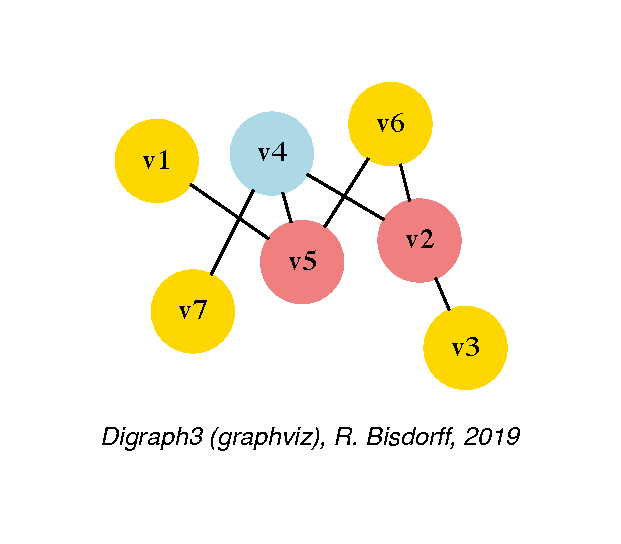
\includegraphics[width=6cm]{Figures/21-2-tutorial-3-coloring.pdf}\hfill
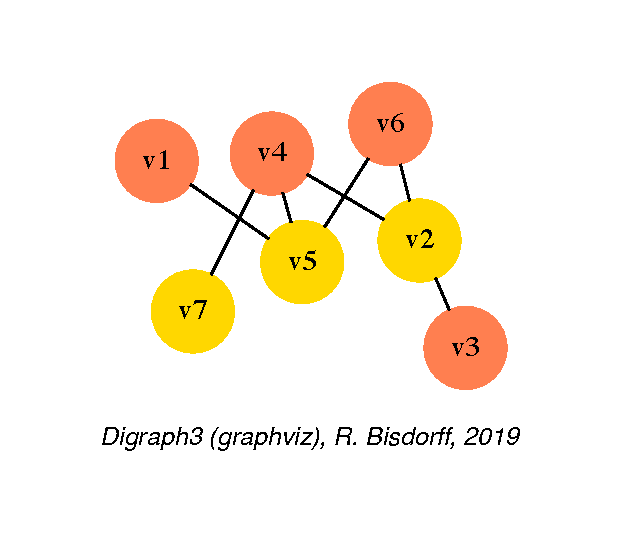
\includegraphics[width=6cm]{Figures/21-2-tutorial-2-coloring.pdf}
\caption{3-Coloring and 2-Coloring of the tutorial graph} 
\label{fig:21.2}       % Give a unique label
\end{figure}

\section{MIS and clique enumeration}
\label{sec:21.3}

2-colorings define sets of independent vertices that are maximal in cardinality --the MISs. The \texttt{showMIS()} method \index{showMIS@\texttt{showMIS()}} computes and prints out such sets. The result is stored in a \texttt{misset} attribute (see Listing~\vref{list:21.6})
\begin{lstlisting}[caption={Computing and printing the maximal independent sets of graph \texttt{g}},label=list:21.6]
>>> g = Graph('tutorialGraph')
>>> g.showMIS()
  *---  Maximal Independent Sets ---*
    ['v2', 'v5', 'v7']
    ['v3', 'v5', 'v7']
    ['v1', 'v2', 'v7']
    ['v1', 'v3', 'v6', 'v7']
    ['v1', 'v3', 'v4', 'v6']
    number of solutions:  5
    cardinality distribution
    card.:  [0, 1, 2, 3, 4, 5, 6, 7]
    freq.:  [0, 0, 0, 3, 2, 0, 0, 0]
    execution time: 0.00032 sec.
    Results in self.misset
>>> g.misset
    [frozenset({'v7', 'v2', 'v5'}), 
     frozenset({'v3', 'v7', 'v5'}), 
     frozenset({'v1', 'v2', 'v7'}), 
     frozenset({'v1', 'v6', 'v7', 'v3'}), 
     frozenset({'v1', 'v6', 'v4', 'v3'})]
\end{lstlisting}

A MIS in the dual \texttt{-g} of a graph instance \texttt{g}, corresponds to a maximal \emph{clique}, i.e. a maximal complete subgraph in \texttt{g}. Maximal cliques may be computed and printed with the \texttt{showCliques()} method\index{showCliques@\texttt{showCliques()}}. The result is stored in a \texttt{clique} attribute as shown in Listing~\vref{list:21.7}.
\begin{lstlisting}[caption={Computing and printing the maximal independent sets of graph \texttt{g}},label=list:21.7]
>>> g.showCliques()
  *---  Maximal Cliques ---*
    ['v2', 'v3']
    ['v4', 'v7']
    ['v2', 'v4']
    ['v4', 'v5']
    ['v1', 'v5']
    ['v2', 'v6']
    ['v5', 'v6']
   number of solutions:  7
   cardinality distribution
   card.:  [0, 1, 2, 3, 4, 5, 6, 7]
   freq.:  [0, 0, 7, 0, 0, 0, 0, 0]
   execution time: 0.00049 sec.
   Results in self.cliques
>>> g.cliques
  [frozenset({'v2', 'v3'}), frozenset({'v4', 'v7'}), 
   frozenset({'v2', 'v4'}), frozenset({'v4', 'v5'}), 
   frozenset({'v1', 'v5'}), frozenset({'v6', 'v2'}), 
   frozenset({'v6', 'v5'})]
\end{lstlisting}

\section{Line graphs and maximal matchings}
\label{sec:21.4}

The \texttt{graphs} module also provides a \texttt{LineGraph}\index{LineGraph@\texttt{LineGraph} class} constructor. A \emph{line graph} represents the adjacencies between edges of the given graph instance. In Listing~\vref{list:21.8} we compute for instance the line graph of the 5-cycle graph.\index{CycleGraph@\texttt{CycleGraph} class}
\begin{lstlisting}[caption={Computing the line graph of the 5-cycle graph},label=list:21.8]
>>> from graphs import CycleGraph, LineGraph
>>> g = CycleGraph(order=5)
>>> g
  *------- Graph instance description ----*
   Instance class   : CycleGraph
   Instance name    : cycleGraph
   Graph Order      : 5
   Graph Size       : 5
   Valuation domain : [-1.00; 1.00]
   Attributes       : ['name', 'order',
             'vertices', 'valuationDomain',
             'edges', 'size', 'gamma']
>>> lg = LineGraph(g)
>>> lg
  *------- Graph instance description ------*
   Instance class   : LineGraph
   Instance name    : line-cycleGraph
   Graph Order      : 5
   Graph Size       : 5
   Valuation domain : [-1.00; 1.00]
   Attributes       : ['name', 'graph',
              'valuationDomain', 'vertices',
               'order', 'edges', 'size', 'gamma']
>>> lg.showShort()
  *---- short description of the graph ----*
   Name             : 'line-cycleGraph'
   Vertices         :  [frozenset({'v1', 'v2'}),
        frozenset({'v1', 'v5'}), frozenset({'v2', 'v3'}),
        frozenset({'v3', 'v4'}), frozenset({'v4', 'v5'})]
   Valuation domain :  {'min': Decimal('-1'),
                'med': Decimal('0'), 'max': Decimal('1')}
   Gamma function   : 
    frozenset({'v1', 'v2'}) ->
         [frozenset({'v2', 'v3'}), frozenset({'v1', 'v5'})]
    frozenset({'v1', 'v5'}) ->
         [frozenset({'v1', 'v2'}), frozenset({'v4', 'v5'})]
    frozenset({'v2', 'v3'}) ->
         [frozenset({'v1', 'v2'}), frozenset({'v3', 'v4'})]
    frozenset({'v3', 'v4'}) ->
         [frozenset({'v2', 'v3'}), frozenset({'v4', 'v5'})]
    frozenset({'v4', 'v5'}) ->
         [frozenset({'v4', 'v3'}), frozenset({'v1', 'v5'})]
   degrees      :  [0, 1, 2, 3, 4]
   distribution :  [0, 0, 5, 0, 0]
   nbh depths   :  [0, 1, 2, 3, 4, 'inf.']
   distribution :  [0, 0, 5, 0, 0, 0]
\end{lstlisting}

Iterated line graph constructions are usually expanding, except for chordless cycles, where the same cycle is repeated, and for non-closed paths, where iterated line graphs progressively reduce one by one the number of vertices and edges and eventually become an empty graph.

Notice in Listing~\vref{list:21.9} that the MISs in a line graph provide \emph{maximal matchings} --maximal sets of independent edges-- of the original graph.
\begin{lstlisting}[caption={Computing the MISs of the line graph of the 8-cycle graph},label=list:21.9,basicstyle=\ttfamily\scriptsize]
>>> c8 = CycleGraph(order=8)
>>> lc8 = LineGraph(c8)
>>> lc8.showMIS()
  *---  Maximal Independent Sets ---*
    [frozenset({'v3', 'v4'}), frozenset({'v5', 'v6'}), frozenset({'v1', 'v8'})]
    [frozenset({'v2', 'v3'}), frozenset({'v5', 'v6'}), frozenset({'v1', 'v8'})]
    [frozenset({'v8', 'v7'}), frozenset({'v2', 'v3'}), frozenset({'v5', 'v6'})]
    [frozenset({'v8', 'v7'}), frozenset({'v2', 'v3'}), frozenset({'v4', 'v5'})]
    [frozenset({'v7', 'v6'}), frozenset({'v3', 'v4'}), frozenset({'v1', 'v8'})]
    [frozenset({'v2', 'v1'}), frozenset({'v8', 'v7'}), frozenset({'v4', 'v5'})]
    [frozenset({'v2', 'v1'}), frozenset({'v7', 'v6'}), frozenset({'v4', 'v5'})]
    [frozenset({'v2', 'v1'}), frozenset({'v7', 'v6'}), frozenset({'v3', 'v4'})]
    [frozenset({'v7', 'v6'}), frozenset({'v2', 'v3'}), frozenset({'v1', 'v8'}),
     frozenset({'v4', 'v5'})]
    [frozenset({'v2', 'v1'}), frozenset({'v8', 'v7'}), frozenset({'v3', 'v4'}),
     frozenset({'v5', 'v6'})]
    number of solutions:  10
    cardinality distribution
    card.:  [0, 1, 2, 3, 4, 5, 6, 7, 8]
    freq.:  [0, 0, 0, 8, 2, 0, 0, 0, 0]
    execution time: 0.00029 sec.
\end{lstlisting}

\begin{figure}[h]
\sidecaption[t]
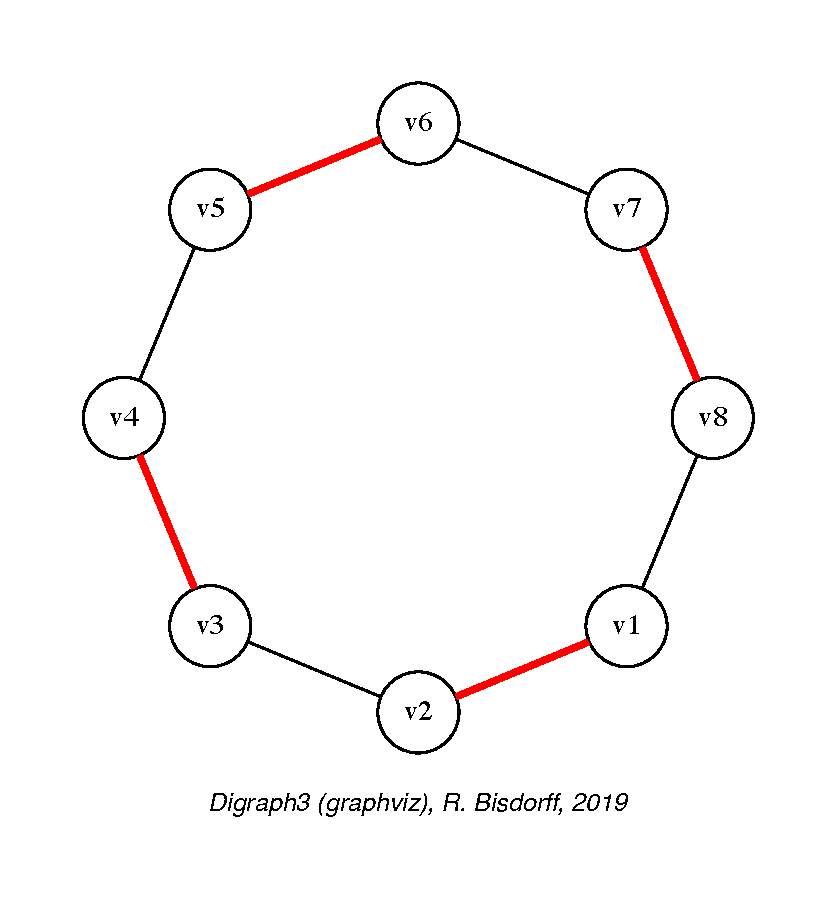
\includegraphics[width=7cm]{Figures/21-3-maxMatchingcycleGraph.pdf}
\caption{A perfect maximum matching of the 8-cycle graph. Every vertex of the 8-cycle is adjacent to a matching edge. Odd cycle graphs do not admit any perfect matching} 
\label{fig:21.3}       % Give a unique label
\end{figure}

The two last MISs of cardinality 4 (see Lines 13-16 in Listing~\vref{list:21.9}) give perfect maximum matchings of the 8-cycle graph as shown in Fig.~\vref{fig:21.3}. 
\begin{lstlisting}[caption={Computing maximum matchings in the 8-cycle graph},label=list:21.10]
>>> maxMatching = c8.computeMaximumMatching()
>>> c8.exportGraphViz(fileName='maxMatchingcycleGraph',\
...   		      matching=maxMatching)
  *---- exporting a dot file for GraphViz tools -----*
   Exporting to maxMatchingcyleGraph.dot
   Matching:  {frozenset({'v1', 'v2'}),
               frozenset({'v5', 'v6'}),
               frozenset({'v3', 'v4'}),
               frozenset({'v7', 'v8'}) }
   circo -Tpng maxMatchingcyleGraph.dot\
                  -o maxMatchingcyleGraph.png
\end{lstlisting}
	    
\section{Grids and the \Ising model}
\label{sec:21.5}

Special classes of graphs, like the \texttt{GridGraph}\index{GridGraph@\texttt{GridGraph} class} class provide $n \times m$ rectangular or triangular grids. With a \emph{Gibbs} sampler\footnote{\citet{GEM-1984}} the \texttt{IsingModel} class\index{IsingModel@\texttt{IsingModel} class} can simulate in Fig.~\vref{fig:21.4} an \Ising model on,for instance, a $15 \times 15$ grid \citep{ISI-1925}.
\begin{lstlisting}[caption={Simulating an Ising model on a the $15 \times 15$ rectangular grid},label=list:21.11]
>>> from graphs import GridGraph, IsingModel
>>> g = GridGraph(n=15,m=15)
>>> g.showShort()
  *----- show short --------------*
   Grid graph    :  grid-6-6
   n             :  6
   m             :  6
   order         :  36
>>> im = IsingModel(g,beta=0.3,nSim=100000)
  Running a Gibbs Sampler for 100000 step !
>>> im.exportGraphViz(colors=['lightblue','lightcoral'])
  *---- exporting a dot file for GraphViz tools ---------*
   Exporting to grid-15-15-ising.dot
   fdp -Tpng grid-15-15-ising.dot -o grid-15-15-ising.png
\end{lstlisting}
\begin{figure}[h]
\sidecaption
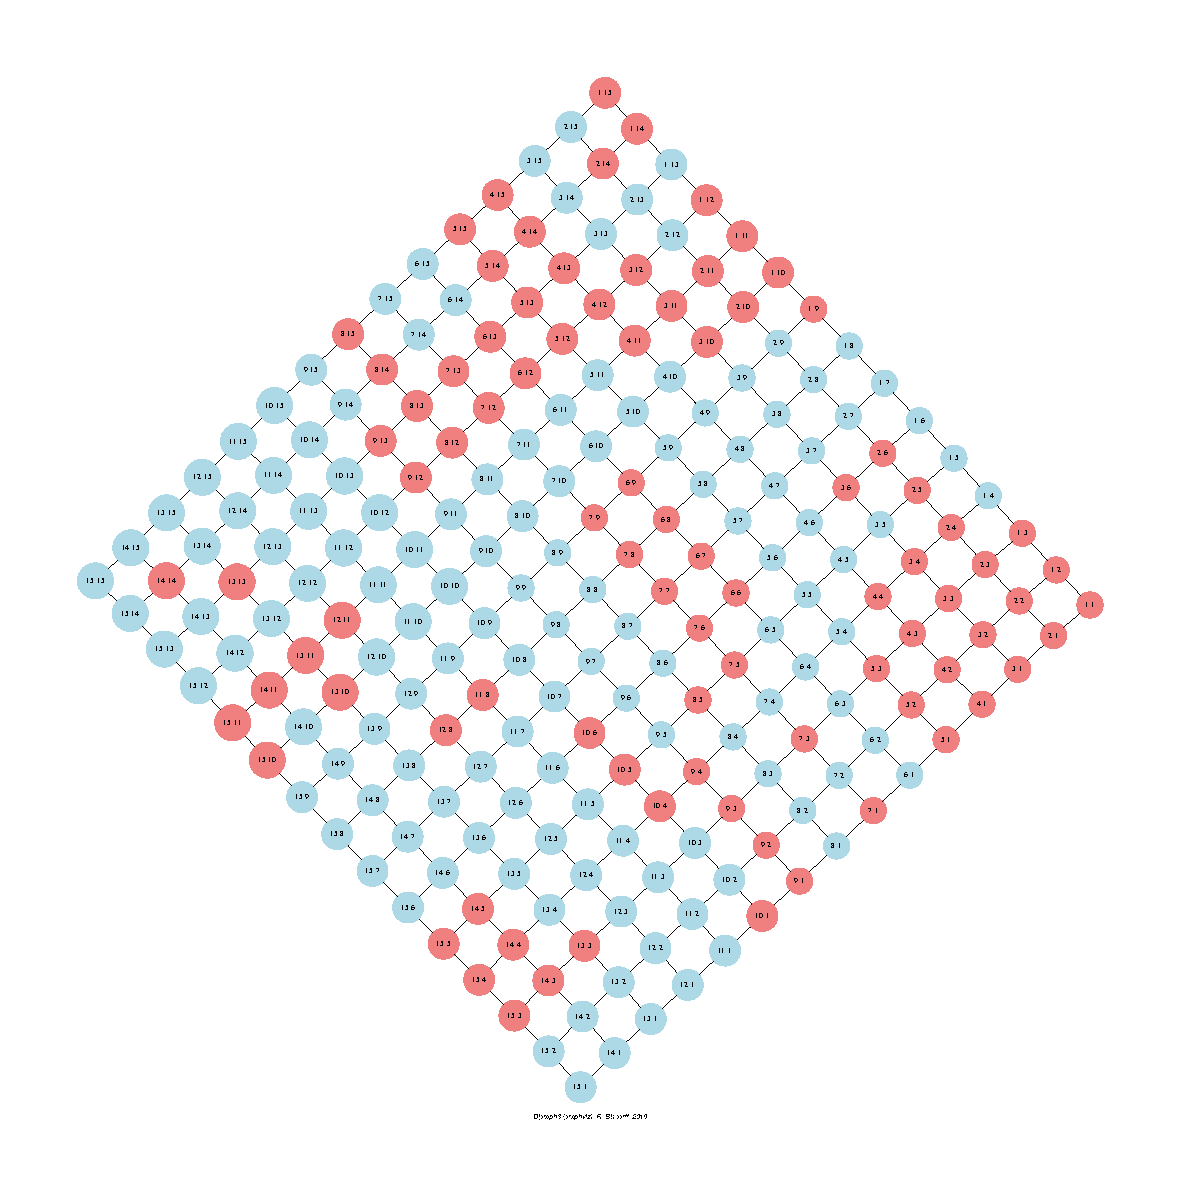
\includegraphics[width=11cm]{Figures/21-4-grid-15-15-ising.pdf}
\caption{Ising model of the 15x15 grid graph.} 
\label{fig:21.4}       % Give a unique label
\end{figure}

\section{Simulating \Metropolis random walks}
\label{sec:21.6}

Finally, we provide the \texttt{MetropolisChain} class\index{MetropolisChain@\texttt{MetropolisChain} class}, a specialization of the \texttt{Graph} class, implementing a generic Monte Carlo Markov Chain (MCMC) sampler for simulating random walks on a graph following given transition probabilities \texttt{probs} = \{\texttt{'v1'}’: $x$, \texttt{'v2'}: $y$, ...\} for visiting each vertex (see Listing~\vref{list:21.12})
\citep{MET-1953}.
\begin{lstlisting}[caption={Simulating random walks on a graph},label=list:21.12]
>>> from graphs import Graph
>>> g = Graph(numberOfVertices=5,edgeProbability=0.5)
>>> g.showShort()
  *---- short description of the graph ----*
   Name             : 'randomGraph'
   Vertices         :  ['v1', 'v2', 'v3', 'v4', 'v5']
   Valuation domain :  {'max': 1, 'med': 0, 'min': -1}
   Gamma function   :
    v1 -> ['v2', 'v3', 'v4']
    v2 -> ['v1', 'v4']
    v3 -> ['v5', 'v1']
    v4 -> ['v2', 'v5', 'v1']
    v5 -> ['v3', 'v4']
>>> # initialize a potential stationary probability vector 
>>> n = g.order
>>> i = 0
>>> for v in g.vertices:
...     probs[v] = (n - i)/(n*(n+1)/2)
...     i += 1
\end{lstlisting}

The \texttt{checkSampling()} method \index{checkSampling@\texttt{checkSampling()}} of the the \texttt{MetropolisChain} class\index{MetropolisChain@\texttt{MetropolisChain} class} (see below) generates a random walk of $nSim = 30000$ steps on the given graph and records by the way the observed relative frequency with which each vertex is passed by. In Listing~\vref{list:21.13} we notice how well the random walk is matching the given stationary probability vector.
\begin{lstlisting}[caption={Checking the quality of the MCMC sampler},label=list:21.13]
>>> from graphs import MetropolisChain     
>>> met = MetropolisChain(g,probs)
>>> frequency = met.checkSampling(verticesList[0],nSim=30000)
>>> for v in verticesList:
...     print(v,probs[v],frequency[v])   
    v1 0.3333 0.3343
    v2 0.2666 0.2680
    v3 0.2    0.2030
    v4 0.1333 0.1311
    v5 0.0666 0.0635
\end{lstlisting}

In this example, the stationary transition probability distribution (see Listing above), shown by the \texttt{showTransitionMatrix()} method\index{showTransitionMatrix@\texttt{showTransitionMatrix()}} in Listing~\vref{list:21.14} is quite adequately simulated.
\begin{lstlisting}[caption={Printing the transition probability distribution},label=list:21.14]
>>> met.showTransitionMatrix()
  * ---- Transition Matrix -----
    Pij  | 'v1'    'v2'    'v3'    'v4'    'v5'
    -----|-------------------------------------
    'v1' |  0.23   0.33    0.30    0.13    0.00
    'v2' |  0.42   0.42    0.00    0.17    0.00
    'v3' |  0.50   0.00    0.33    0.00    0.17
    'v4' |  0.33   0.33    0.00    0.08    0.25
    'v5' |  0.00   0.00    0.50    0.50    0.00
\end{lstlisting}

For the reader interested in algorithmic applications of Markov Chains we recommend consulting \citet{HAG-2002}.

%%%%%%%%%
\section{Computing the non isomorphic MISs of the n-cycle graph}
\label{sec:21.7}

Due to the public success of our common work with Jean-Luc Marichal \citep{ISO-2008}, we present in this chapter an example Python session for computing the non isomorphic maximal independent sets (MISs) of the 12-cycle graph, i.e. a \texttt{CirculantDigraph} class\index{CirculantDigraph@\texttt{CirculantDigraph} class} instance of order 12 and symmetric circulants $1$ and $-1$.
\begin{lstlisting}
>>> from digraphs import CirculantDigraph
>>> c12 = CirculantDigraph(order=12,circulants=[1,-1])
>>> c12 # 12-cycle digraph instance
  *------- Digraph instance description ------*
   Instance class   : CirculantDigraph
   Instance name    : c12
   Digraph Order    : 12
   Digraph Size     : 24
   Valuation domain : [-1.0, 1.0]
   Determinateness  : 100.000
   Attributes       : ['name', 'order', 'circulants',
                       'actions', 'valuationdomain',
                       'relation', 'gamma', 'notGamma']
\end{lstlisting}

Such $n$-cycle graphs -- see the 12-cycle graph in Fig,~\vref{fig:21.5}-- are also provided as undirected graph instances by the \texttt{CycleGraph} class.\index{CycleGraph@\texttt{CycleGraph} class}
\begin{lstlisting}
>>> from graphs import CycleGraph
>>> cg12 = CycleGraph(order=12)
>>> cg12
  *------- Graph instance description ------*
   Instance class   : CycleGraph
   Instance name    : cycleGraph
   Graph Order      : 12
   Graph Size       : 12
   Valuation domain : [-1.0, 1.0]
   Attributes       : ['name', 'order', 'vertices',
                       'valuationDomain', 'edges',
                       'size', 'gamma']
% >>> cg12.exportGraphViz('cg12')
% \end{lstlisting}
% \begin{figure}[h]
% \sidecaption[t]
% 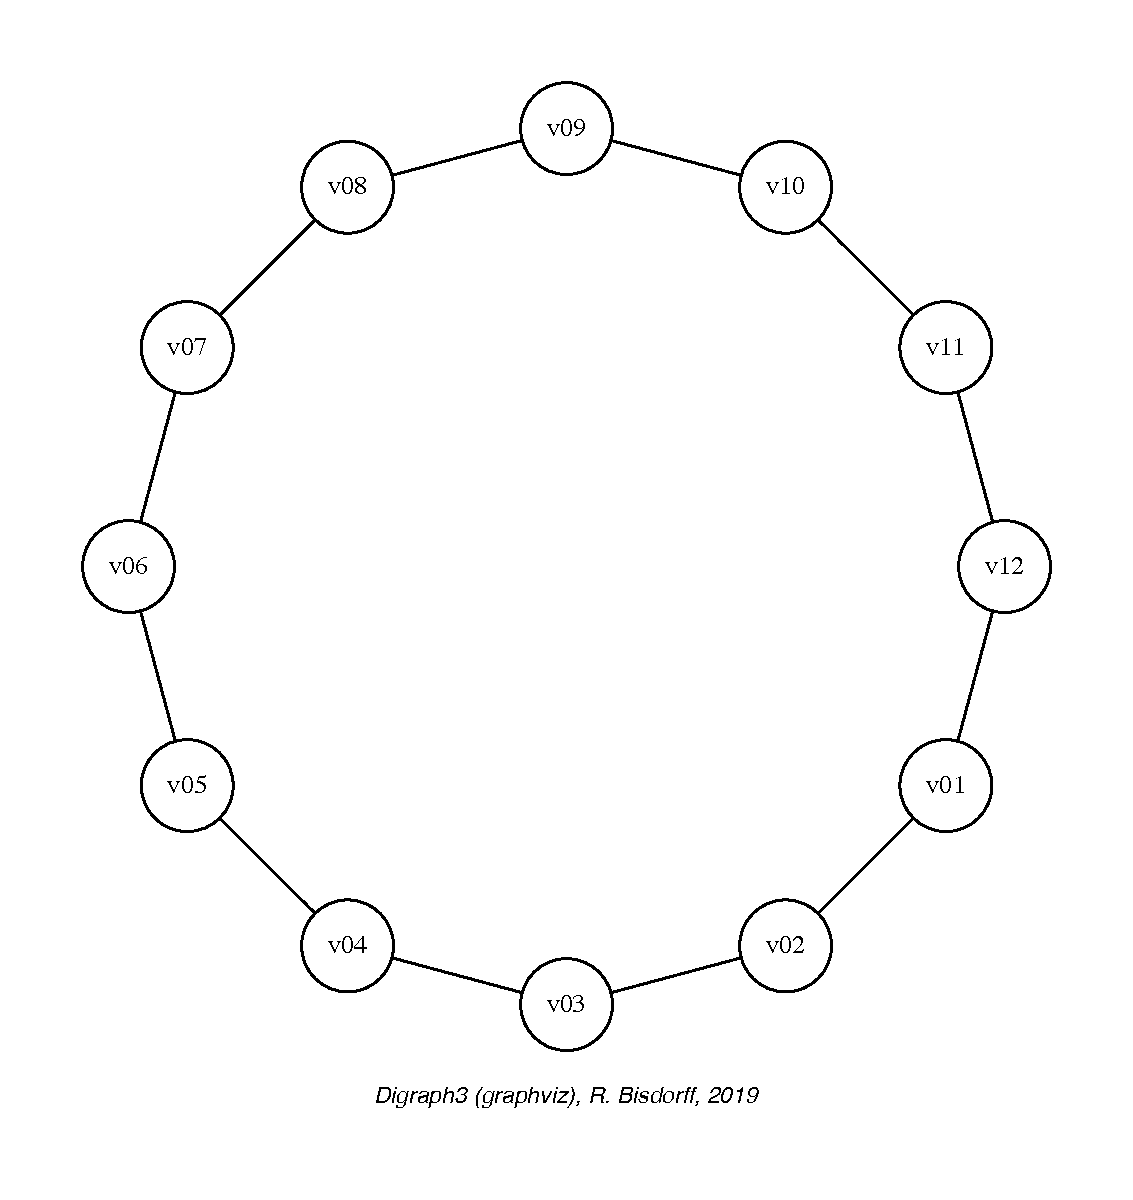
\includegraphics[width=6cm]{Figures/21-5-cg12.pdf}
% \caption{The 12-cycle graph} 
% \label{fig:21.5}       % Give a unique label
% \end{figure}

% \subsection{Computing maximal independent sets (MISs)}
% \label{sec:21.7.1}

A non-isomorphic MIS of the 12-cycle graph corresponds in fact to a set of isomorphic MISs, i.e. an orbit of MISs under the automorphism group of the 12-cycle graph. In Listing~\vref{list:21.15} we are now first computing all maximal independent sets that are detectable in the 12-cycle digraph with the \texttt{showMIS()} method.
\begin{lstlisting}[caption={Computing the MISs of the 12-cycle graph},label=list:21.15]
>>> c12.showMIS(withListing=False)
  *---  Maximal independent choices ---*
   number of solutions:  29
   cardinality distribution
   card.:  [0, 1, 2, 3, 4,  5,  6, 7, 8, 9, 10, 11, 12]
   freq.:  [0, 0, 0, 0, 3, 24,  2, 0, 0, 0,  0,  0,  0]
   Results in c12.misset
\end{lstlisting}
In the 12-cycle graph, we observe 29 labelled MISs: 3 of cardinality 4, 24 of cardinality 5, and 2  of cardinality 6. In case of n-cycle graphs with $n > 20$, as the cardinality of the MISs becomes big, it is preferable to use, as shown in Listing~\vref{list:21.16}, the \texttt{perrinMIS} shall command\index{perrinMIS@\texttt{perrinMIS} shell command}\footnote{The \texttt{perrinMIS} shell command may be installed system wide with the command texttt{make installPerrin} from the main \Digraph directory. It is stored by default into \texttt{/usr/local/bin/}. This may be changed with the \texttt{INSTALLDIR} flag. The command \texttt{make installPerrinUser} installs it instead without sudo into the user's private \texttt{.bin} directory.} compiled from C and installed  along with all the \Digraph python modules for computing the set of MISs observed in the graph.
\begin{lstlisting}[caption={Computing the MISs with the \texttt{perrinMIS} shell command},label=list:21.16]
...$ echo 12 | /usr/local/bin/perrinMIS
  # $------------------------------------- #
  # Generating MIS set of Cn with the      #
  # Perrin sequence algorithm.             #
  # Temporary files used.                  #
  # even versus odd order optimised.       #
  # RB December 2006                       #
  # Current revision Dec 2018              #
  # -------------------------------------- #
  Input cycle order ? <-- 12
   mis 1 : 100100100100
   mis 2 : 010010010010
   mis 3 : 001001001001
    ...
    ...
    ...
   mis 27 : 001001010101
   mis 28 : 101010101010
   mis 29 : 010101010101
   Cardinalities:
   0 : 0
   1 : 0
   2 : 0
   3 : 0
   4 : 3
   5 : 24
   6 : 2
   7 : 0
   8 : 0
   9 : 0
   10 : 0
   11 : 0
   12 : 0
   Total: 29
   execution time: 0 sec. and 2 millisec.
\end{lstlisting}
Reading in the result of the \texttt{perrinMIS} shell command, stored in a file called by default \texttt{curd.dat}, may be operated with the \texttt{readPerrinMisset()} method \index{readPerrinMisset@\texttt{readPerrinMisset()}}.
\begin{lstlisting}
>>> c12.readPerrinMisset(file='curd.dat')
>>> c12.misset
    {frozenset({'5', '7', '10', '1', '3'}),
     frozenset({'9', '11', '5', '2', '7'}),
     frozenset({'7', '2', '4', '10', '12'}),
     ...
     ...
     ...
     frozenset({'8', '4', '10', '1', '6'}),
     frozenset({'11', '4', '1', '9', '6'}),
     frozenset({'8', '2', '4', '10', '12', '6'})
    }
\end{lstlisting}

For computing the corresponding non-isomorphic MISs, we actually need the automorphism group of the 12-cycle graph. The \texttt{Digraph} class therefore provides the \texttt{automorphismGenerators()} method\index{automorphismGenerators@\texttt{automorphismGenerators()}} which adds automorphism group generators to a \texttt{Digraph} class instance with the help of the external shell \texttt{dreadnaut} shell command\index{dreadnaut@\texttt{dreadnaut} shell command} from the \emph{nauty} software package \footnote{The \texttt{automorphismGenerators} method uses the \texttt{dreadnaut} shell command from the \emph{nauty} software package. See https://www3.cs.stonybrook.edu/~algorith/implement/nauty/implement.shtml . On Mac OS there exist dmg installers and on Ubuntu Linux or Debian, one may easily install it with \texttt{...\$ sudo apt-get install nauty}.}.
\begin{lstlisting}[caption={Computing the automorphism group generators},label=list:21.17]
>>> c12.automorphismGenerators()
      ...
    Permutations
    {'1':'1', '2':'12', '3':'11', '4':'10',
     '5':'9', '6':'8', '7':'7', '8':'6', '9':'5',
     '10':'4', '11':'3', '12':'2'}
    {'1':'2', '2':'1', '3':'12', '4':'11', '5':'10', 
     '6':'9', '7':'8', '8':'7', '9':'6', '10':'5', 
     '11':'4', '12':'3'}
>>> print('grpsize = ', c12.automorphismGroupSize)
   grpsize = 24
\end{lstlisting}
The 12-cycle graph's automorphism group, of size 24, is generated with both the permutations shown in Listing~\vref{list:21.17}.

The \texttt{showOrbits()} method renders now the labelled representatives of each of the four orbits of isomorphic MISs observed in the 12-cycle graph (see Lines 7-10 below).
\begin{lstlisting}[caption={Computing the MISs orbits of the 12-cycle graph},label=list:21.18]
>>> c12.showOrbits(c12.misset,withListing=False)
    ...
  *---- Global result ----
   Number of MIS:  29
   Number of orbits :  4
   Labelled representatives and cardinality:
   1: ['2','4','6','8','10','12'], 2
   2: ['2','5','8','11'], 3
   3: ['2','4','6','9','11'], 12
   4: ['1','4','7','9','11'], 12
   Symmetry vector
   stabilizer size: [1, 2, 3, ..., 8, 9, ..., 12, 13, ...]
   frequency      : [0, 2, 0, ..., 1, 0, ...,  1,  0, ...]
\end{lstlisting}
The corresponding group stabilizers' sizes and frequencies: orbit 1 with 6 symmetry axes, orbit 2 with 4 symmetry axes, and orbits 3 and 4 both with one symmetry axis (see Lines 12-13 in Listing~\vref{list:21.18}), are illustrated in the corresponding unlabelled graphs of Fig.~\vref{fig:21.5}.
\begin{figure}[h]
\sidecaption[t]
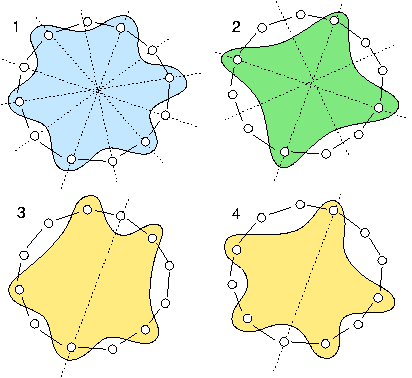
\includegraphics[width=6cm]{Figures/21-5-c12.png}
\caption{The symmetry axes of the four non isomorphic MISs of the 12-cycle graph} 
\label{fig:21.5}       % Give a unique label
\end{figure}

The non isomorphic MISs in the 12-cycle graph represent in fact all the ways one may write the number 12 as the circular sum of '2's and '3's without distinguishing opposite directions of writing. The first orbit corresponds to writing six times a '2'; the second orbit corresponds to writing four times a '3'. The third and fourth orbit correspond to writing two times a '3' and three times a '2'. There are two non isomorphic ways to do this latter circular sum. Either separating the '3's by one and two '2's, or by zero and three '2's \citep{ISO-2008}.

\vspace{1cm}

\noindent The next chapter is devoted more specifically to tree graphs and graph forests.

%%%%%%% The chapter bibliography
%\normallatexbib
\clearpage
%\phantomsection
%\addcontentsline{toc}{section}{Chapter Bibliography}
\bibliographystyle{spbasic}
\typeout{}
\bibliography{03-backMatters/reference}
%\chapter{Working with undirected graphs}
\label{sec:22}

\abstract*{}

\abstract{}

\section{Implementing undirected graphs}
\label{sec:22.1}

In the \Digraph {\tt graphs} module, the root \texttt{Graph} class provides a generic simple graph model, without loops and multiple links. A given object of this class contains at least the following attributes in:
\begin{enumerate}
\item \texttt{vertices}: a dictionary of vertices with \texttt{name} and \texttt{shortName} attributes,
\item \texttt{edges} : a dictionary with \emph{frozensets} \footnote{\href{https://docs.python.org/3.9/library/stdtypes.html?highlight=frozenset\#frozenset}{Python documentation}} of pairs of vertices as entries carrying a characteristic value in the range of the previous valuation domain,
\item \texttt{valuationDomain}: a dictionary with three entries: the minimum ($-1$, means certainly no link), the median ($0$, means missing information) and the maximum characteristic value ($+1$, means certainly a link),
\item \texttt{gamma}: a dictionary containing the direct neighbors of each vertex, automatically added by the object constructor.
\end{enumerate}

Example Python3 session:
\begin{lstlisting}
>>> from graphs import Graph
>>> g = Graph(numberOfVertices=7,edgeProbability=0.5)
>>> g.save(fileName='tutorialGraph')
\end{lstlisting}

The saved \texttt{Graph} instance named \texttt{tutorialGraph.py} is encoded as follows.
\begin{lstlisting}
    # Graph instance saved in Python format
    vertices = {
    'v1': {'shortName': 'v1', 'name': 'random vertex'},
    'v2': {'shortName': 'v2', 'name': 'random vertex'},
    'v3': {'shortName': 'v3', 'name': 'random vertex'},
    'v4': {'shortName': 'v4', 'name': 'random vertex'},
    'v5': {'shortName': 'v5', 'name': 'random vertex'},
    'v6': {'shortName': 'v6', 'name': 'random vertex'},
    'v7': {'shortName': 'v7', 'name': 'random vertex'},
    }
    valuationDomain = {'min':-1,'med':0,'max':1}
    edges = {
    frozenset(['v1','v2']) : -1, 
    frozenset(['v1','v3']) : -1, 
    frozenset(['v1','v4']) : -1, 
    frozenset(['v1','v5']) : 1, 
    frozenset(['v1','v6']) : -1, 
    frozenset(['v1','v7']) : -1, 
    frozenset(['v2','v3']) : 1, 
    frozenset(['v2','v4']) : 1, 
    frozenset(['v2','v5']) : -1, 
    frozenset(['v2','v6']) : 1, 
    frozenset(['v2','v7']) : -1, 
    frozenset(['v3','v4']) : -1, 
    frozenset(['v3','v5']) : -1, 
    frozenset(['v3','v6']) : -1, 
    frozenset(['v3','v7']) : -1, 
    frozenset(['v4','v5']) : 1, 
    frozenset(['v4','v6']) : -1, 
    frozenset(['v4','v7']) : 1, 
    frozenset(['v5','v6']) : 1, 
    frozenset(['v5','v7']) : -1, 
    frozenset(['v6','v7']) : -1, 
    }
\end{lstlisting}

The stored graph can be reloaded and plotted with the generic \\
\texttt{exportGraphViz()} Footnote[1] method as follows:
\begin{lstlisting}
>>> g = Graph('tutorialGraph')
>>> g.exportGraphViz()
  *---- exporting a dot file for GraphViz tools ---------*
   Exporting to tutorialGraph.dot
   fdp -Tpng tutorialGraph.dot -o tutorialGraph.png
\end{lstlisting}
\begin{figure}[h]
\sidecaption
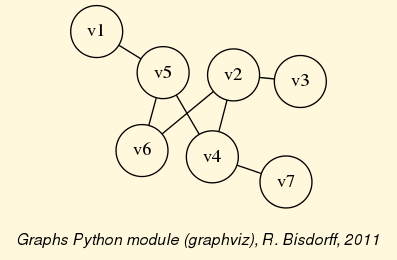
\includegraphics[width=7cm]{Figures/tutorialGraph.png}
\caption{Example simple graph instance} 
\label{fig:22.1}       % Give a unique label
\end{figure}

Properties, like the gamma function and vertex degrees and neighbourhood depths may be shown with a \texttt{showShort()} method.
\begin{lstlisting}
>>> g.showShort()
  *---- short description of the graph ----*
   Name : 'tutorialGraph'
   Vertices :  ['v1','v2','v3','v4','v5','v6','v7']
   Valuation domain : {'min': -1, 'med': 0, 'max': 1}
   Gamma function   : 
    v1 -> ['v5']
    v2 -> ['v6', 'v4', 'v3']
    v3 -> ['v2']
    v4 -> ['v5', 'v2', 'v7']
    v5 -> ['v1', 'v6', 'v4']
    v6 -> ['v2', 'v5']
    v7 -> ['v4']
   degrees      :  [0, 1, 2, 3, 4, 5, 6]
   distribution :  [0, 3, 1, 3, 0, 0, 0]
   nbh depths   :  [0, 1, 2, 3, 4, 5, 6, 'inf.']
   distribution :  [0, 0, 1, 4, 2, 0, 0, 0]
\end{lstlisting}

A \texttt{Graph} instance corresponds bijectively to a symmetric \texttt{Digraph} instance and we may easily convert from one to the other with the \texttt{graph2Digraph()}, and vice versa with the \texttt{digraph2Graph()} method. Thus, all computing resources of the \texttt{Digraph} class, suitable for symmetric digraphs, become readily available, and vice versa.
\begin{lstlisting}
>>> dg = g.graph2Digraph()
>>> dg.showRelationTable(ndigits=0,ReflexiveTerms=False)
  * ---- Relation Table -----
    S  |  'v1'  'v2'  'v3'  'v4'  'v5'  'v6'  'v7'	  
  -----|------------------------------------------
  'v1' |    -    -1    -1    -1     1    -1    -1	 
  'v2' |   -1     -     1     1    -1     1    -1	 
  'v3' |   -1     1     -    -1    -1    -1    -1	 
  'v4' |   -1     1    -1     -     1    -1     1	 
  'v5' |    1    -1    -1     1     -     1    -1	 
  'v6' |   -1     1    -1    -1     1     -    -1	 
  'v7' |   -1    -1    -1     1    -1    -1     -
>>> g1 = dg.digraph2Graph()
>>> g1.showShort()
  *---- short description of the graph ----*
   Name         : 'tutorialGraph'
   Vertices     :  ['v1','v2','v3','v4','v5','v6','v7']
   Valuation domain :   {'med': 0, 'min': -1, 'max': 1}
   Gamma function   : 
    v1 -> ['v5']
    v2 -> ['v3', 'v6', 'v4']
    v3 -> ['v2']
    v4 -> ['v5', 'v7', 'v2']
    v5 -> ['v6', 'v1', 'v4']
    v6 -> ['v5', 'v2']
    v7 -> ['v4']
   degrees      :  [0, 1, 2, 3, 4, 5, 6]
   distribution :  [0, 3, 1, 3, 0, 0, 0]
   nbh depths   :  [0, 1, 2, 3, 4, 5, 6, 'inf.']
   distribution :  [0, 0, 1, 4, 2, 0, 0, 0]
\end{lstlisting}

\section{q-coloring of a graph}
\label{25.2}

A 3-coloring of the tutorial graph $g$ may for instance be computed and plotted with the \texttt{Q\_Coloring} class as follows.
\begin{lstlisting}
>>> from graphs import Q_Coloring
>>> qc = Q_Coloring(g)
  Running a Gibbs Sampler for 42 step !
  The q-coloring with 3 colors is feasible !!
>>> qc.showConfiguration()
    v5 lightblue
    v3 gold
    v7 gold
    v2 lightblue
    v4 lightcoral
    v1 gold
    v6 lightcoral
>>> qc.exportGraphViz('tutorial-3-coloring')
  *---- exporting a dot file for GraphViz tools
   Exporting to tutorial-3-coloring.dot
   fdp -Tpng tutorial-3-coloring.dot\
                    -o tutorial-3-coloring.png
\end{lstlisting}
\begin{figure}[h]
\sidecaption
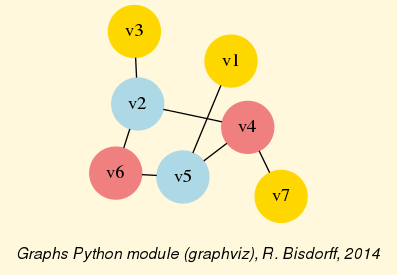
\includegraphics[width=7cm]{Figures/tutorial-3-coloring.png}
\caption{3-Coloring of the tutorial graph} 
\label{fig:22.2}       % Give a unique label
\end{figure}

Actually, with the given tutorial graph instance, a 2-coloring is already feasible.
\begin{lstlisting}
>>> qc = Q_Coloring(g,colors=['gold','coral'])
  Running a Gibbs Sampler for 42 step !
  The q-coloring with 2 colors is feasible !!
>>> qc.showConfiguration()
    v5 gold
    v3 coral
    v7 gold
    v2 gold
    v4 coral
    v1 coral
    v6 coral
>>> qc.exportGraphViz('tutorial-2-coloring')
  Exporting to tutorial-2-coloring.dot
  fdp -Tpng tutorial-2-coloring.dot\
                    -o tutorial-2-coloring.png
\end{lstlisting}
\begin{figure}[h]
\sidecaption
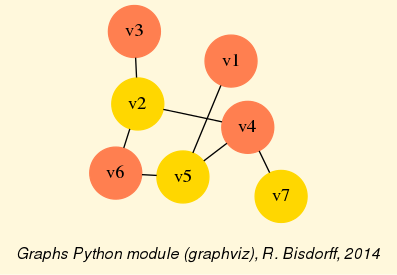
\includegraphics[width=7cm]{Figures/tutorial-2-coloring.png}
\caption{3-Coloring of the tutorial graph} 
\label{fig:22.3}       % Give a unique label
\end{figure}

\section{MIS and clique enumeration}
\label{sec:22.3}

2-colorings define independent sets of vertices that are maximal in cardinality. Computing such MISs in a given \texttt{Graph} instance may be achieved by the \texttt{showMIS} method.
\begin{lstlisting}
>>> g = Graph('tutorialGraph')
>>> g.showMIS()
  *---  Maximal Independent Sets ---*
    ['v2', 'v5', 'v7']
    ['v3', 'v5', 'v7']
    ['v1', 'v2', 'v7']
    ['v1', 'v3', 'v6', 'v7']
    ['v1', 'v3', 'v4', 'v6']
    number of solutions:  5
    cardinality distribution
    card.:  [0, 1, 2, 3, 4, 5, 6, 7]
    freq.:  [0, 0, 0, 3, 2, 0, 0, 0]
    execution time: 0.00032 sec.
    Results in self.misset
>>> g.misset
    [frozenset({'v7', 'v2', 'v5'}), 
     frozenset({'v3', 'v7', 'v5'}), 
     frozenset({'v1', 'v2', 'v7'}), 
     frozenset({'v1', 'v6', 'v7', 'v3'}), 
     frozenset({'v1', 'v6', 'v4', 'v3'})]
\end{lstlisting}

A MIS in the dual of a graph instance $g$, corresponds to a maximal \emph{clique}, i.e. a maximal complete subgraph in $g$. Maximal cliques may be directly enumerated with the \texttt{showCliques()} method.
\begin{lstlisting}
>>> g.showCliques()
  *---  Maximal Cliques ---*
    ['v2', 'v3']
    ['v4', 'v7']
    ['v2', 'v4']
    ['v4', 'v5']
    ['v1', 'v5']
    ['v2', 'v6']
    ['v5', 'v6']
   number of solutions:  7
   cardinality distribution
   card.:  [0, 1, 2, 3, 4, 5, 6, 7]
   freq.:  [0, 0, 7, 0, 0, 0, 0, 0]
   execution time: 0.00049 sec.
   Results in self.cliques
>>> g.cliques
  [frozenset({'v2', 'v3'}), frozenset({'v4', 'v7'}), 
   frozenset({'v2', 'v4'}), frozenset({'v4', 'v5'}), 
   frozenset({'v1', 'v5'}), frozenset({'v6', 'v2'}), 
   frozenset({'v6', 'v5'})]
\end{lstlisting}

\section{Line graphs and maximal matchings}
\label{sec:22.4}

The \texttt{graphs} module also provides a \texttt{LineGraph} constructor. A \emph{line graph} represents the adjacencies between edges of the given graph instance. We may compute for instance the line graph of the 5-cycle graph.
\begin{lstlisting}
>>> from graphs import CycleGraph, LineGraph
>>> g = CycleGraph(order=5)
>>> g
  *------- Graph instance description ----*
   Instance class   : CycleGraph
   Instance name    : cycleGraph
   Graph Order      : 5
   Graph Size       : 5
   Valuation domain : [-1.00; 1.00]
   Attributes       : ['name', 'order',
             'vertices', 'valuationDomain',
             'edges', 'size', 'gamma']
>>> lg = LineGraph(g)
>>> lg
  *------- Graph instance description ------*
   Instance class   : LineGraph
   Instance name    : line-cycleGraph
   Graph Order      : 5
   Graph Size       : 5
   Valuation domain : [-1.00; 1.00]
   Attributes       : ['name', 'graph',
              'valuationDomain', 'vertices',
               'order', 'edges', 'size', 'gamma']
>>> lg.showShort()
  *---- short description of the graph ----*
   Name             : 'line-cycleGraph'
   Vertices         :  [frozenset({'v1', 'v2'}),
        frozenset({'v1', 'v5'}), frozenset({'v2', 'v3'}),
        frozenset({'v3', 'v4'}), frozenset({'v4', 'v5'})]
   Valuation domain :  {'min': Decimal('-1'),
                'med': Decimal('0'), 'max': Decimal('1')}
   Gamma function   : 
    frozenset({'v1', 'v2'}) ->
         [frozenset({'v2', 'v3'}), frozenset({'v1', 'v5'})]
    frozenset({'v1', 'v5'}) ->
         [frozenset({'v1', 'v2'}), frozenset({'v4', 'v5'})]
    frozenset({'v2', 'v3'}) ->
         [frozenset({'v1', 'v2'}), frozenset({'v3', 'v4'})]
    frozenset({'v3', 'v4'}) ->
         [frozenset({'v2', 'v3'}), frozenset({'v4', 'v5'})]
    frozenset({'v4', 'v5'}) ->
         [frozenset({'v4', 'v3'}), frozenset({'v1', 'v5'})]
   degrees      :  [0, 1, 2, 3, 4]
   distribution :  [0, 0, 5, 0, 0]
   nbh depths   :  [0, 1, 2, 3, 4, 'inf.']
   distribution :  [0, 0, 5, 0, 0, 0]
\end{lstlisting}

Iterated line graph constructions are usually expanding, except for chordless cycles, where the same cycle is repeated, and for non-closed paths, where iterated line graphs progressively reduce one by one the number of vertices and edges and become eventually an empty graph.

Notice that the MISs in the line graph provide \emph{maximal matchings} --maximal sets of independent edges-- of the original graph.
\begin{lstlisting}[basicstyle=\scriptsize]
>>> c8 = CycleGraph(order=8)
>>> lc8 = LineGraph(c8)
>>> lc8.showMIS()
  *---  Maximal Independent Sets ---*
    [frozenset({'v3', 'v4'}), frozenset({'v5', 'v6'}), frozenset({'v1', 'v8'})]
    [frozenset({'v2', 'v3'}), frozenset({'v5', 'v6'}), frozenset({'v1', 'v8'})]
    [frozenset({'v8', 'v7'}), frozenset({'v2', 'v3'}), frozenset({'v5', 'v6'})]
    [frozenset({'v8', 'v7'}), frozenset({'v2', 'v3'}), frozenset({'v4', 'v5'})]
    [frozenset({'v7', 'v6'}), frozenset({'v3', 'v4'}), frozenset({'v1', 'v8'})]
    [frozenset({'v2', 'v1'}), frozenset({'v8', 'v7'}), frozenset({'v4', 'v5'})]
    [frozenset({'v2', 'v1'}), frozenset({'v7', 'v6'}), frozenset({'v4', 'v5'})]
    [frozenset({'v2', 'v1'}), frozenset({'v7', 'v6'}), frozenset({'v3', 'v4'})]
    [frozenset({'v7', 'v6'}), frozenset({'v2', 'v3'}), frozenset({'v1', 'v8'}),
     frozenset({'v4', 'v5'})]
    [frozenset({'v2', 'v1'}), frozenset({'v8', 'v7'}), frozenset({'v3', 'v4'}),
     frozenset({'v5', 'v6'})]
    number of solutions:  10
    cardinality distribution
    card.:  [0, 1, 2, 3, 4, 5, 6, 7, 8]
    freq.:  [0, 0, 0, 8, 2, 0, 0, 0, 0]
    execution time: 0.00029 sec.
\end{lstlisting}
The two last MISs of cardinality 4 (see Lines 13-16 above) give isomorphic perfect maximum matchings of the 8-cycle graph. Every vertex of the cycle is adjacent to a matching edge. Odd cycle graphs do not admit any perfect matching.
\begin{lstlisting}
>>> maxMatching = c8.computeMaximumMatching()
>>> c8.exportGraphViz(fileName='maxMatchingcycleGraph',\
...   		      matching=maxMatching)
  *---- exporting a dot file for GraphViz tools -----*
   Exporting to maxMatchingcyleGraph.dot
   Matching:  {frozenset({'v1', 'v2'}),
               frozenset({'v5', 'v6'}),
               frozenset({'v3', 'v4'}),
               frozenset({'v7', 'v8'}) }
   circo -Tpng maxMatchingcyleGraph.dot\
                  -o maxMatchingcyleGraph.png
\end{lstlisting}
\begin{figure}[h]
\sidecaption
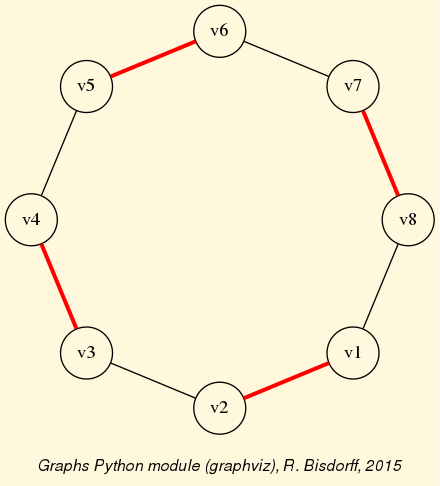
\includegraphics[width=7cm]{Figures/maxMatchingcycleGraph.png}
\caption{A perfect maximum matching of the 8-cycle graph} 
\label{fig:22.4}       % Give a unique label
\end{figure}
	    
\section{Grids and the Ising model}
\label{sec:22.5}

Special classes of graphs, like $n \times m$ rectangular or triangular grids (\texttt{GridGraph} and \texttt{IsingModel}) are available from the \texttt{graphs} module. For instance, we may use a \emph{Gibbs} sampler again for simulating an \emph{Ising Model} on such a grid.
\begin{lstlisting}
>>> from graphs import GridGraph, IsingModel
>>> g = GridGraph(n=15,m=15)
>>> g.showShort()
  *----- show short --------------*
   Grid graph    :  grid-6-6
   n             :  6
   m             :  6
   order         :  36
>>> im = IsingModel(g,beta=0.3,nSim=100000,Debug=False)
  Running a Gibbs Sampler for 100000 step !
>>> im.exportGraphViz(colors=['lightblue','lightcoral'])
  *---- exporting a dot file for GraphViz tools ---------*
   Exporting to grid-15-15-ising.dot
   fdp -Tpng grid-15-15-ising.dot -o grid-15-15-ising.png
\end{lstlisting}
\begin{figure}[h]
\sidecaption
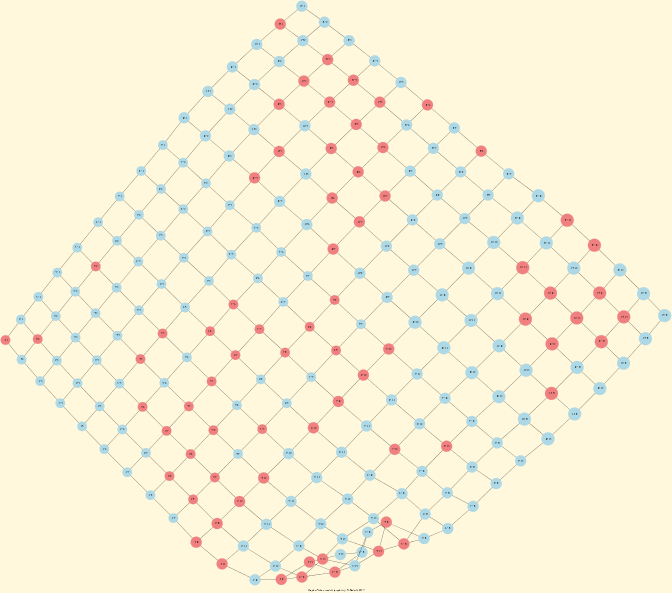
\includegraphics[width=11cm]{Figures/grid-15-15-ising.png}
\caption{Ising model of the 15x15 grid graph} 
\label{fig:22.5}       % Give a unique label
\end{figure}

\section{Simulating Metropolis random walks}
\label{sec:22.6}

Finally, we provide the \texttt{MetropolisChain} class, a specialization of the \texttt{Graph} class, for implementing a generic \emph{Metropolis} Monte Carlo Markov Chain (MCMC) sampler for simulating random walks on a given graph $g$:
\begin{lstlisting}
>>> from graphs import Graph
>>> g = Graph(numberOfVertices=5,edgeProbability=0.5)
>>> g.showShort()
  *---- short description of the graph ----*
   Name             : 'randomGraph'
   Vertices         :  ['v1', 'v2', 'v3', 'v4', 'v5']
   Valuation domain :  {'max': 1, 'med': 0, 'min': -1}
   Gamma function   :
    v1 -> ['v2', 'v3', 'v4']
    v2 -> ['v1', 'v4']
    v3 -> ['v5', 'v1']
    v4 -> ['v2', 'v5', 'v1']
    v5 -> ['v3', 'v4']
\end{lstlisting}
following a given probability $probs$ = \{‘v1’: $x$, ‘v2’: $y$, ...\} for visiting each vertex:
\begin{lstlisting}
>>> probs = {}  # initialize a potential stationary probability vector 
>>> n = g.order # for instance: probs[v_i] = n-i/Sum(1:n) for i in 1:n
>>> i = 0
>>> verticesList = [x for x in g.vertices]
>>> verticesList.sort()
>>> for v in verticesList:
...     probs[v] = (n - i)/(n*(n+1)/2)
...     i += 1
\end{lstlisting}

The \texttt{checkSampling()} method of the the \texttt{MetropolisChain} class (see below) generates a random walk of $nSim = 30000$ steps on the given graph and records by the way the observed relative frequency with which each vertex is passed by:
\begin{lstlisting}
>>> from graphs import MetropolisChain     
>>> met = MetropolisChain(g,probs)
>>> frequency = met.checkSampling(verticesList[0],nSim=30000)
>>> for v in verticesList:
...     print(v,probs[v],frequency[v])   
    v1 0.3333 0.3343
    v2 0.2666 0.2680
    v3 0.2    0.2030
    v4 0.1333 0.1311
    v5 0.0666 0.0635
\end{lstlisting}
  In this example, the stationary transition probability distribution (see Listing above), shown by the \texttt{showTransitionMatrix()} method below is quite adequately simulated.
\begin{lstlisting}
>>> met.showTransitionMatrix()
  * ---- Transition Matrix -----
    Pij  | 'v1'    'v2'    'v3'    'v4'    'v5'
    -----|-------------------------------------
    'v1' |  0.23   0.33    0.30    0.13    0.00
    'v2' |  0.42   0.42    0.00    0.17    0.00
    'v3' |  0.50   0.00    0.33    0.00    0.17
    'v4' |  0.33   0.33    0.00    0.08    0.25
    'v5' |  0.00   0.00    0.50    0.50    0.00
\end{lstlisting}

For the reader interested in algorithmic applications of Markov Chains we may recommend consulting O. Häggström's 2002 book: \citep{FMCAA}.

%%%%%%%%%
\section[The n-cycle graph]{Computing the non isomorphic MISs of the n-cycle graph}
\label{sec:22.7}

Due to the public success of our common 2008 publication with Jean-Luc Marichal \citep{ISOMIS-08} , we present in this chapter an example Python session for computing the non isomorphic maximal independent sets (MISs) from the 12-cycle graph, i.e. a \texttt{CirculantDigraph} class instance of order 12 and symmetric circulants $1$ and $-1$.
\begin{lstlisting}
>>> from digraphs import CirculantDigraph
>>> c12 = CirculantDigraph(order=12,circulants=[1,-1])
>>> c12 # 12-cycle digraph instance
  *------- Digraph instance description ------*
   Instance class   : CirculantDigraph
   Instance name    : c12
   Digraph Order    : 12
   Digraph Size     : 24
   Valuation domain : [-1.0, 1.0]
   Determinateness  : 100.000
   Attributes       : ['name', 'order', 'circulants',
                       'actions', 'valuationdomain',
                       'relation', 'gamma', 'notGamma']
\end{lstlisting}

Such $n$-cycle graphs are also provided as undirected graph instances by the \texttt{CycleGraph} class.
\begin{lstlisting}
>>> from graphs import CycleGraph
>>> cg12 = CycleGraph(order=12)
>>> cg12
  *------- Graph instance description ------*
   Instance class   : CycleGraph
   Instance name    : cycleGraph
   Graph Order      : 12
   Graph Size       : 12
   Valuation domain : [-1.0, 1.0]
   Attributes       : ['name', 'order', 'vertices',
                       'valuationDomain', 'edges',
                       'size', 'gamma']
>>> cg12.exportGraphViz('cg12')
\end{lstlisting}
\begin{figure}[h]
\sidecaption[t]
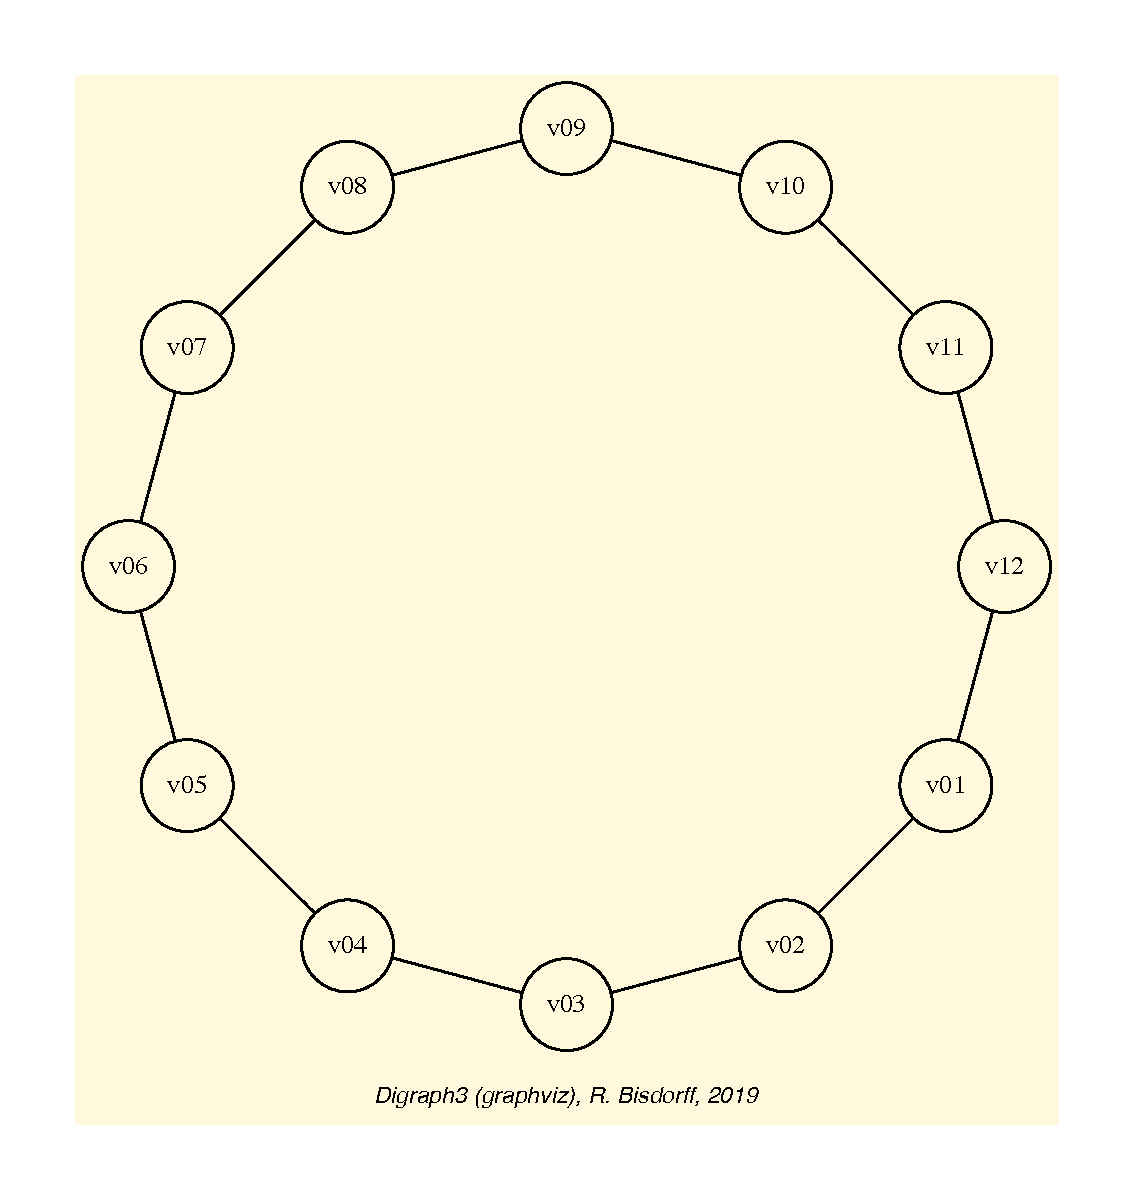
\includegraphics[width=6cm]{Figures/cg12.pdf}
\caption{The 12-cycle graph} 
\label{fig:22.7.1}       % Give a unique label
\end{figure}

\subsection{Computing maximal independent sets (MISs)}
\label{sec:22.7.1}

A non isomorphic MIS corresponds in fact to a set of isomorphic MISs, i.e. an orbit of MISs under the automorphism group of the 12-cycle graph. We are now first computing all maximal independent sets that are detectable in the 12-cycle digraph with the \texttt{showMIS()} method.
\begin{lstlisting}
>>> c12.showMIS(withListing=False)
  *---  Maximal independent choices ---*
   number of solutions:  29
   cardinality distribution
   card.:  [0, 1, 2, 3, 4,  5,  6, 7, 8, 9, 10, 11, 12]
   freq.:  [0, 0, 0, 0, 3, 24,  2, 0, 0, 0,  0,  0,  0]
   Results in c12.misset
\end{lstlisting}
In the 12-cycle graph, we observe 29 labelled MISs: 3 of cardinality 4, 24 of cardinality 5, and 2  of cardinality 6. In case of n-cycle graphs with $n$ > 20, as the cardinality of the MISs becomes big, it is preferable to use the \texttt{perrinMIS} shall command\index{perrinMIS@\texttt{perrinMIS} shell command} compiled from C and installed  along with all the \Digraph python modules for computing the set of MISs observed in the graph\footnote{The \texttt{perrinMIS} shell command may be installed system wide with the command texttt{make installPerrin} from the main \Digraph directory. It is stored by default into \texttt{/usr/local/bin/}. This may be changed with the \texttt{INSTALLDIR} flag. The command \texttt{make installPerrinUser} installs it instead without sudo into the user's private \texttt{.bin} directory.}.
\begin{lstlisting}
...$ echo 12 | /usr/local/bin/perrinMIS
  # $------------------------------------- #
  # Generating MIS set of Cn with the      #
  # Perrin sequence algorithm.             #
  # Temporary files used.                  #
  # even versus odd order optimised.       #
  # RB December 2006                       #
  # Current revision Dec 2018              #
  # -------------------------------------- #
  Input cycle order ? <-- 12
   mis 1 : 100100100100
   mis 2 : 010010010010
   mis 3 : 001001001001
    ...
    ...
    ...
   mis 27 : 001001010101
   mis 28 : 101010101010
   mis 29 : 010101010101
   Cardinalities:
   0 : 0
   1 : 0
   2 : 0
   3 : 0
   4 : 3
   5 : 24
   6 : 2
   7 : 0
   8 : 0
   9 : 0
   10 : 0
   11 : 0
   12 : 0
   Total: 29
   execution time: 0 sec. and 2 millisec.
\end{lstlisting}
Reading in the result of the \texttt{perrinMIS} shell command, stored in a file called by default \texttt{curd.dat}, may be operated with the \texttt{readPerrinMisset()} method \index{readPerrinMisset@\texttt{readPerrinMisset()}}.
\begin{lstlisting}
>>> c12.readPerrinMisset(file='curd.dat')
>>> c12.misset
    {frozenset({'5', '7', '10', '1', '3'}),
     frozenset({'9', '11', '5', '2', '7'}),
     frozenset({'7', '2', '4', '10', '12'}),
     ...
     ...
     ...
     frozenset({'8', '4', '10', '1', '6'}),
     frozenset({'11', '4', '1', '9', '6'}),
     frozenset({'8', '2', '4', '10', '12', '6'})
    }
\end{lstlisting}

\subsection{Computing the automorphism group}
\label{sec:22.7.2}

For computing the corresponding non isomorphic MISs, we actually need the automorphism group of the c12-cycle graph. The \texttt{Digraph} class therefore provides the \texttt{automorphismGenerators()} method\index{automorphismGenerators@\texttt{automorphismGenerators()}} which adds automorphism group generators to a \texttt{Digraph} class instance with the help of the external shell \texttt{dreadnaut} shell command\index{dreadnaut@\texttt{dreadnaut} shell command} from the \emph{nauty} software package \footnote{The \texttt{automorphismGenerators} method uses the \texttt{dreadnaut} shell command from the \emph{nauty} software package. See https://www3.cs.stonybrook.edu/~algorith/implement/nauty/implement.shtml . On Mac OS there exist dmg installers and on Ubuntu Linux or Debian, one may easily install it with \texttt{...\$ sudo apt-get install nauty}.}.
\begin{lstlisting}
>>> c12.automorphismGenerators()
      ...
    Permutations
    {'1':'1', '2':'12', '3':'11', '4':'10',
     '5':'9', '6':'8', '7':'7', '8':'6', '9':'5',
     '10':'4', '11':'3', '12':'2'}
    {'1':'2', '2':'1', '3':'12', '4':'11', '5':'10', 
     '6':'9', '7':'8', '8':'7', '9':'6', '10':'5', 
     '11':'4', '12':'3'}
>>> print('grpsize = ', c12.automorphismGroupSize)
   grpsize = 24
\end{lstlisting}
The 12-cycle graph automorphism group is generated with both the permutations above and has group size 24.

\subsection{Computing the isomorphic MISs}
\label{sec:22.7.3}

The \texttt{showOrbits()} method renders now the labelled representatives of each of the four orbits of isomorphic MISs observed in the 12-cycle graph (see Lines 7-10 below).
\begin{lstlisting}
>>> c12.showOrbits(c12.misset,withListing=False)
    ...
  *---- Global result ----
   Number of MIS:  29
   Number of orbits :  4
   Labelled representatives and cardinality:
   1: ['2','4','6','8','10','12'], 2
   2: ['2','5','8','11'], 3
   3: ['2','4','6','9','11'], 12
   4: ['1','4','7','9','11'], 12
   Symmetry vector
   stabilizer size: [1, 2, 3, ..., 8, 9, ..., 12, 13, ...]
   frequency      : [0, 2, 0, ..., 1, 0, ...,  1,  0, ...]
\end{lstlisting}
The corresponding group stabilizers' sizes and frequencies: orbit 1 with 6 symmetry axes, orbit 2 with 4 symmetry axes, and orbits 3 and 4 both with one symmetry axis (see Lines 12-13 above), are illustrated in the corresponding unlabelled graphs of Fig.~\ref{fig:22.7.2} below.
\begin{figure}[h]
\sidecaption[t]
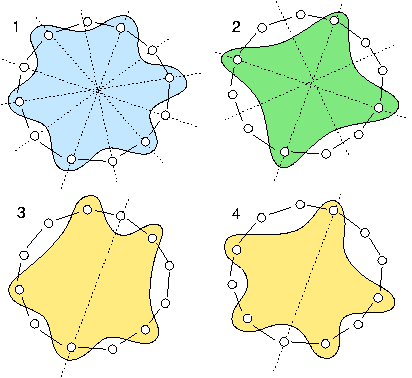
\includegraphics[width=6cm]{Figures/c12.png}
\caption{The symmetry axes of the four non isomorphic MISs of the 12-cycle graph} 
\label{fig:22.7.2}       % Give a unique label
\end{figure}

The non isomorphic MISs in the 12-cycle graph represent in fact all the ways one may write the number 12 as the circular sum of '2's and '3's without distinguishing opposite directions of writing. The first orbit corresponds to writing six times a '2'; the second orbit corresponds to writing four times a '3'. The third and fourth orbit correspond to writing two times a '3' and three times a '2'. There are two non isomorphic ways to do this latter circular sum. Either separating the '3's by one and two '2's, or by zero and three '2's (see \citep{ISOMIS-08}).


%%%%%%% The chapter bibliography
%\normallatexbib
\clearpage
%\phantomsection
%\addcontentsline{toc}{section}{Chapter Bibliography}
\bibliographystyle{spbasic}
\typeout{}
\bibliography{03-backMatters/reference}
%\chapter{Working with undirected graphs}
\label{sec:22}

\abstract*{}

\abstract{}

\section{Implementing undirected graphs}
\label{sec:22.1}

In the \Digraph {\tt graphs} module, the root \texttt{Graph} class provides a generic simple graph model, without loops and multiple links. A given object of this class contains at least the following attributes in:
\begin{enumerate}
\item \texttt{vertices}: a dictionary of vertices with \texttt{name} and \texttt{shortName} attributes,
\item \texttt{edges} : a dictionary with \emph{frozensets} \footnote{\href{https://docs.python.org/3.9/library/stdtypes.html?highlight=frozenset\#frozenset}{Python documentation}} of pairs of vertices as entries carrying a characteristic value in the range of the previous valuation domain,
\item \texttt{valuationDomain}: a dictionary with three entries: the minimum ($-1$, means certainly no link), the median ($0$, means missing information) and the maximum characteristic value ($+1$, means certainly a link),
\item \texttt{gamma}: a dictionary containing the direct neighbors of each vertex, automatically added by the object constructor.
\end{enumerate}

Example Python3 session:
\begin{lstlisting}
>>> from graphs import Graph
>>> g = Graph(numberOfVertices=7,edgeProbability=0.5)
>>> g.save(fileName='tutorialGraph')
\end{lstlisting}

The saved \texttt{Graph} instance named \texttt{tutorialGraph.py} is encoded as follows.
\begin{lstlisting}
    # Graph instance saved in Python format
    vertices = {
    'v1': {'shortName': 'v1', 'name': 'random vertex'},
    'v2': {'shortName': 'v2', 'name': 'random vertex'},
    'v3': {'shortName': 'v3', 'name': 'random vertex'},
    'v4': {'shortName': 'v4', 'name': 'random vertex'},
    'v5': {'shortName': 'v5', 'name': 'random vertex'},
    'v6': {'shortName': 'v6', 'name': 'random vertex'},
    'v7': {'shortName': 'v7', 'name': 'random vertex'},
    }
    valuationDomain = {'min':-1,'med':0,'max':1}
    edges = {
    frozenset(['v1','v2']) : -1, 
    frozenset(['v1','v3']) : -1, 
    frozenset(['v1','v4']) : -1, 
    frozenset(['v1','v5']) : 1, 
    frozenset(['v1','v6']) : -1, 
    frozenset(['v1','v7']) : -1, 
    frozenset(['v2','v3']) : 1, 
    frozenset(['v2','v4']) : 1, 
    frozenset(['v2','v5']) : -1, 
    frozenset(['v2','v6']) : 1, 
    frozenset(['v2','v7']) : -1, 
    frozenset(['v3','v4']) : -1, 
    frozenset(['v3','v5']) : -1, 
    frozenset(['v3','v6']) : -1, 
    frozenset(['v3','v7']) : -1, 
    frozenset(['v4','v5']) : 1, 
    frozenset(['v4','v6']) : -1, 
    frozenset(['v4','v7']) : 1, 
    frozenset(['v5','v6']) : 1, 
    frozenset(['v5','v7']) : -1, 
    frozenset(['v6','v7']) : -1, 
    }
\end{lstlisting}

The stored graph can be reloaded and plotted with the generic \\
\texttt{exportGraphViz()} Footnote[1] method as follows:
\begin{lstlisting}
>>> g = Graph('tutorialGraph')
>>> g.exportGraphViz()
  *---- exporting a dot file for GraphViz tools ---------*
   Exporting to tutorialGraph.dot
   fdp -Tpng tutorialGraph.dot -o tutorialGraph.png
\end{lstlisting}
\begin{figure}[h]
\sidecaption
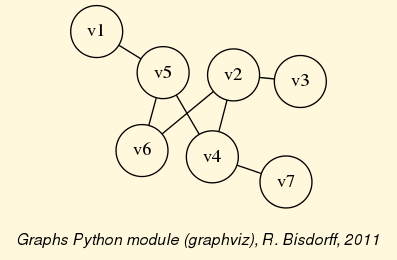
\includegraphics[width=7cm]{Figures/tutorialGraph.png}
\caption{Example simple graph instance} 
\label{fig:22.1}       % Give a unique label
\end{figure}

Properties, like the gamma function and vertex degrees and neighbourhood depths may be shown with a \texttt{showShort()} method.
\begin{lstlisting}
>>> g.showShort()
  *---- short description of the graph ----*
   Name : 'tutorialGraph'
   Vertices :  ['v1','v2','v3','v4','v5','v6','v7']
   Valuation domain : {'min': -1, 'med': 0, 'max': 1}
   Gamma function   : 
    v1 -> ['v5']
    v2 -> ['v6', 'v4', 'v3']
    v3 -> ['v2']
    v4 -> ['v5', 'v2', 'v7']
    v5 -> ['v1', 'v6', 'v4']
    v6 -> ['v2', 'v5']
    v7 -> ['v4']
   degrees      :  [0, 1, 2, 3, 4, 5, 6]
   distribution :  [0, 3, 1, 3, 0, 0, 0]
   nbh depths   :  [0, 1, 2, 3, 4, 5, 6, 'inf.']
   distribution :  [0, 0, 1, 4, 2, 0, 0, 0]
\end{lstlisting}

A \texttt{Graph} instance corresponds bijectively to a symmetric \texttt{Digraph} instance and we may easily convert from one to the other with the \texttt{graph2Digraph()}, and vice versa with the \texttt{digraph2Graph()} method. Thus, all computing resources of the \texttt{Digraph} class, suitable for symmetric digraphs, become readily available, and vice versa.
\begin{lstlisting}
>>> dg = g.graph2Digraph()
>>> dg.showRelationTable(ndigits=0,ReflexiveTerms=False)
  * ---- Relation Table -----
    S  |  'v1'  'v2'  'v3'  'v4'  'v5'  'v6'  'v7'	  
  -----|------------------------------------------
  'v1' |    -    -1    -1    -1     1    -1    -1	 
  'v2' |   -1     -     1     1    -1     1    -1	 
  'v3' |   -1     1     -    -1    -1    -1    -1	 
  'v4' |   -1     1    -1     -     1    -1     1	 
  'v5' |    1    -1    -1     1     -     1    -1	 
  'v6' |   -1     1    -1    -1     1     -    -1	 
  'v7' |   -1    -1    -1     1    -1    -1     -
>>> g1 = dg.digraph2Graph()
>>> g1.showShort()
  *---- short description of the graph ----*
   Name         : 'tutorialGraph'
   Vertices     :  ['v1','v2','v3','v4','v5','v6','v7']
   Valuation domain :   {'med': 0, 'min': -1, 'max': 1}
   Gamma function   : 
    v1 -> ['v5']
    v2 -> ['v3', 'v6', 'v4']
    v3 -> ['v2']
    v4 -> ['v5', 'v7', 'v2']
    v5 -> ['v6', 'v1', 'v4']
    v6 -> ['v5', 'v2']
    v7 -> ['v4']
   degrees      :  [0, 1, 2, 3, 4, 5, 6]
   distribution :  [0, 3, 1, 3, 0, 0, 0]
   nbh depths   :  [0, 1, 2, 3, 4, 5, 6, 'inf.']
   distribution :  [0, 0, 1, 4, 2, 0, 0, 0]
\end{lstlisting}

\section{q-coloring of a graph}
\label{25.2}

A 3-coloring of the tutorial graph $g$ may for instance be computed and plotted with the \texttt{Q\_Coloring} class as follows.
\begin{lstlisting}
>>> from graphs import Q_Coloring
>>> qc = Q_Coloring(g)
  Running a Gibbs Sampler for 42 step !
  The q-coloring with 3 colors is feasible !!
>>> qc.showConfiguration()
    v5 lightblue
    v3 gold
    v7 gold
    v2 lightblue
    v4 lightcoral
    v1 gold
    v6 lightcoral
>>> qc.exportGraphViz('tutorial-3-coloring')
  *---- exporting a dot file for GraphViz tools
   Exporting to tutorial-3-coloring.dot
   fdp -Tpng tutorial-3-coloring.dot\
                    -o tutorial-3-coloring.png
\end{lstlisting}
\begin{figure}[h]
\sidecaption
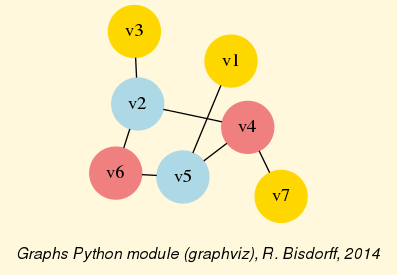
\includegraphics[width=7cm]{Figures/tutorial-3-coloring.png}
\caption{3-Coloring of the tutorial graph} 
\label{fig:22.2}       % Give a unique label
\end{figure}

Actually, with the given tutorial graph instance, a 2-coloring is already feasible.
\begin{lstlisting}
>>> qc = Q_Coloring(g,colors=['gold','coral'])
  Running a Gibbs Sampler for 42 step !
  The q-coloring with 2 colors is feasible !!
>>> qc.showConfiguration()
    v5 gold
    v3 coral
    v7 gold
    v2 gold
    v4 coral
    v1 coral
    v6 coral
>>> qc.exportGraphViz('tutorial-2-coloring')
  Exporting to tutorial-2-coloring.dot
  fdp -Tpng tutorial-2-coloring.dot\
                    -o tutorial-2-coloring.png
\end{lstlisting}
\begin{figure}[h]
\sidecaption
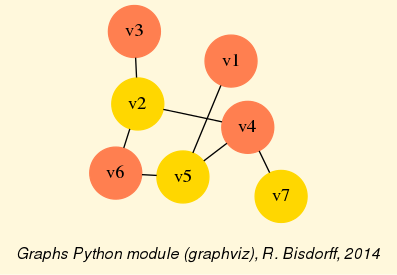
\includegraphics[width=7cm]{Figures/tutorial-2-coloring.png}
\caption{3-Coloring of the tutorial graph} 
\label{fig:22.3}       % Give a unique label
\end{figure}

\section{MIS and clique enumeration}
\label{sec:22.3}

2-colorings define independent sets of vertices that are maximal in cardinality. Computing such MISs in a given \texttt{Graph} instance may be achieved by the \texttt{showMIS} method.
\begin{lstlisting}
>>> g = Graph('tutorialGraph')
>>> g.showMIS()
  *---  Maximal Independent Sets ---*
    ['v2', 'v5', 'v7']
    ['v3', 'v5', 'v7']
    ['v1', 'v2', 'v7']
    ['v1', 'v3', 'v6', 'v7']
    ['v1', 'v3', 'v4', 'v6']
    number of solutions:  5
    cardinality distribution
    card.:  [0, 1, 2, 3, 4, 5, 6, 7]
    freq.:  [0, 0, 0, 3, 2, 0, 0, 0]
    execution time: 0.00032 sec.
    Results in self.misset
>>> g.misset
    [frozenset({'v7', 'v2', 'v5'}), 
     frozenset({'v3', 'v7', 'v5'}), 
     frozenset({'v1', 'v2', 'v7'}), 
     frozenset({'v1', 'v6', 'v7', 'v3'}), 
     frozenset({'v1', 'v6', 'v4', 'v3'})]
\end{lstlisting}

A MIS in the dual of a graph instance $g$, corresponds to a maximal \emph{clique}, i.e. a maximal complete subgraph in $g$. Maximal cliques may be directly enumerated with the \texttt{showCliques()} method.
\begin{lstlisting}
>>> g.showCliques()
  *---  Maximal Cliques ---*
    ['v2', 'v3']
    ['v4', 'v7']
    ['v2', 'v4']
    ['v4', 'v5']
    ['v1', 'v5']
    ['v2', 'v6']
    ['v5', 'v6']
   number of solutions:  7
   cardinality distribution
   card.:  [0, 1, 2, 3, 4, 5, 6, 7]
   freq.:  [0, 0, 7, 0, 0, 0, 0, 0]
   execution time: 0.00049 sec.
   Results in self.cliques
>>> g.cliques
  [frozenset({'v2', 'v3'}), frozenset({'v4', 'v7'}), 
   frozenset({'v2', 'v4'}), frozenset({'v4', 'v5'}), 
   frozenset({'v1', 'v5'}), frozenset({'v6', 'v2'}), 
   frozenset({'v6', 'v5'})]
\end{lstlisting}

\section{Line graphs and maximal matchings}
\label{sec:22.4}

The \texttt{graphs} module also provides a \texttt{LineGraph} constructor. A \emph{line graph} represents the adjacencies between edges of the given graph instance. We may compute for instance the line graph of the 5-cycle graph.
\begin{lstlisting}
>>> from graphs import CycleGraph, LineGraph
>>> g = CycleGraph(order=5)
>>> g
  *------- Graph instance description ----*
   Instance class   : CycleGraph
   Instance name    : cycleGraph
   Graph Order      : 5
   Graph Size       : 5
   Valuation domain : [-1.00; 1.00]
   Attributes       : ['name', 'order',
             'vertices', 'valuationDomain',
             'edges', 'size', 'gamma']
>>> lg = LineGraph(g)
>>> lg
  *------- Graph instance description ------*
   Instance class   : LineGraph
   Instance name    : line-cycleGraph
   Graph Order      : 5
   Graph Size       : 5
   Valuation domain : [-1.00; 1.00]
   Attributes       : ['name', 'graph',
              'valuationDomain', 'vertices',
               'order', 'edges', 'size', 'gamma']
>>> lg.showShort()
  *---- short description of the graph ----*
   Name             : 'line-cycleGraph'
   Vertices         :  [frozenset({'v1', 'v2'}),
        frozenset({'v1', 'v5'}), frozenset({'v2', 'v3'}),
        frozenset({'v3', 'v4'}), frozenset({'v4', 'v5'})]
   Valuation domain :  {'min': Decimal('-1'),
                'med': Decimal('0'), 'max': Decimal('1')}
   Gamma function   : 
    frozenset({'v1', 'v2'}) ->
         [frozenset({'v2', 'v3'}), frozenset({'v1', 'v5'})]
    frozenset({'v1', 'v5'}) ->
         [frozenset({'v1', 'v2'}), frozenset({'v4', 'v5'})]
    frozenset({'v2', 'v3'}) ->
         [frozenset({'v1', 'v2'}), frozenset({'v3', 'v4'})]
    frozenset({'v3', 'v4'}) ->
         [frozenset({'v2', 'v3'}), frozenset({'v4', 'v5'})]
    frozenset({'v4', 'v5'}) ->
         [frozenset({'v4', 'v3'}), frozenset({'v1', 'v5'})]
   degrees      :  [0, 1, 2, 3, 4]
   distribution :  [0, 0, 5, 0, 0]
   nbh depths   :  [0, 1, 2, 3, 4, 'inf.']
   distribution :  [0, 0, 5, 0, 0, 0]
\end{lstlisting}

Iterated line graph constructions are usually expanding, except for chordless cycles, where the same cycle is repeated, and for non-closed paths, where iterated line graphs progressively reduce one by one the number of vertices and edges and become eventually an empty graph.

Notice that the MISs in the line graph provide \emph{maximal matchings} --maximal sets of independent edges-- of the original graph.
\begin{lstlisting}[basicstyle=\scriptsize]
>>> c8 = CycleGraph(order=8)
>>> lc8 = LineGraph(c8)
>>> lc8.showMIS()
  *---  Maximal Independent Sets ---*
    [frozenset({'v3', 'v4'}), frozenset({'v5', 'v6'}), frozenset({'v1', 'v8'})]
    [frozenset({'v2', 'v3'}), frozenset({'v5', 'v6'}), frozenset({'v1', 'v8'})]
    [frozenset({'v8', 'v7'}), frozenset({'v2', 'v3'}), frozenset({'v5', 'v6'})]
    [frozenset({'v8', 'v7'}), frozenset({'v2', 'v3'}), frozenset({'v4', 'v5'})]
    [frozenset({'v7', 'v6'}), frozenset({'v3', 'v4'}), frozenset({'v1', 'v8'})]
    [frozenset({'v2', 'v1'}), frozenset({'v8', 'v7'}), frozenset({'v4', 'v5'})]
    [frozenset({'v2', 'v1'}), frozenset({'v7', 'v6'}), frozenset({'v4', 'v5'})]
    [frozenset({'v2', 'v1'}), frozenset({'v7', 'v6'}), frozenset({'v3', 'v4'})]
    [frozenset({'v7', 'v6'}), frozenset({'v2', 'v3'}), frozenset({'v1', 'v8'}),
     frozenset({'v4', 'v5'})]
    [frozenset({'v2', 'v1'}), frozenset({'v8', 'v7'}), frozenset({'v3', 'v4'}),
     frozenset({'v5', 'v6'})]
    number of solutions:  10
    cardinality distribution
    card.:  [0, 1, 2, 3, 4, 5, 6, 7, 8]
    freq.:  [0, 0, 0, 8, 2, 0, 0, 0, 0]
    execution time: 0.00029 sec.
\end{lstlisting}
The two last MISs of cardinality 4 (see Lines 13-16 above) give isomorphic perfect maximum matchings of the 8-cycle graph. Every vertex of the cycle is adjacent to a matching edge. Odd cycle graphs do not admit any perfect matching.
\begin{lstlisting}
>>> maxMatching = c8.computeMaximumMatching()
>>> c8.exportGraphViz(fileName='maxMatchingcycleGraph',\
...   		      matching=maxMatching)
  *---- exporting a dot file for GraphViz tools -----*
   Exporting to maxMatchingcyleGraph.dot
   Matching:  {frozenset({'v1', 'v2'}),
               frozenset({'v5', 'v6'}),
               frozenset({'v3', 'v4'}),
               frozenset({'v7', 'v8'}) }
   circo -Tpng maxMatchingcyleGraph.dot\
                  -o maxMatchingcyleGraph.png
\end{lstlisting}
\begin{figure}[h]
\sidecaption
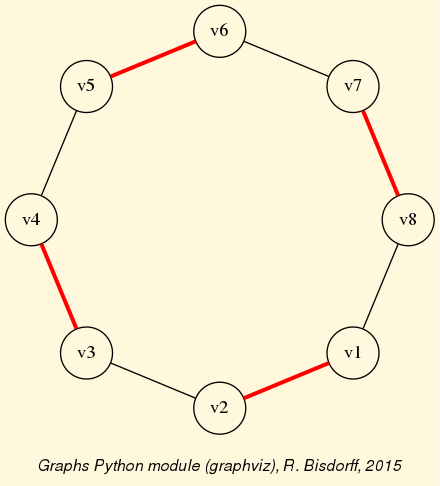
\includegraphics[width=7cm]{Figures/maxMatchingcycleGraph.png}
\caption{A perfect maximum matching of the 8-cycle graph} 
\label{fig:22.4}       % Give a unique label
\end{figure}
	    
\section{Grids and the Ising model}
\label{sec:22.5}

Special classes of graphs, like $n \times m$ rectangular or triangular grids (\texttt{GridGraph} and \texttt{IsingModel}) are available from the \texttt{graphs} module. For instance, we may use a \emph{Gibbs} sampler again for simulating an \emph{Ising Model} on such a grid.
\begin{lstlisting}
>>> from graphs import GridGraph, IsingModel
>>> g = GridGraph(n=15,m=15)
>>> g.showShort()
  *----- show short --------------*
   Grid graph    :  grid-6-6
   n             :  6
   m             :  6
   order         :  36
>>> im = IsingModel(g,beta=0.3,nSim=100000,Debug=False)
  Running a Gibbs Sampler for 100000 step !
>>> im.exportGraphViz(colors=['lightblue','lightcoral'])
  *---- exporting a dot file for GraphViz tools ---------*
   Exporting to grid-15-15-ising.dot
   fdp -Tpng grid-15-15-ising.dot -o grid-15-15-ising.png
\end{lstlisting}
\begin{figure}[h]
\sidecaption
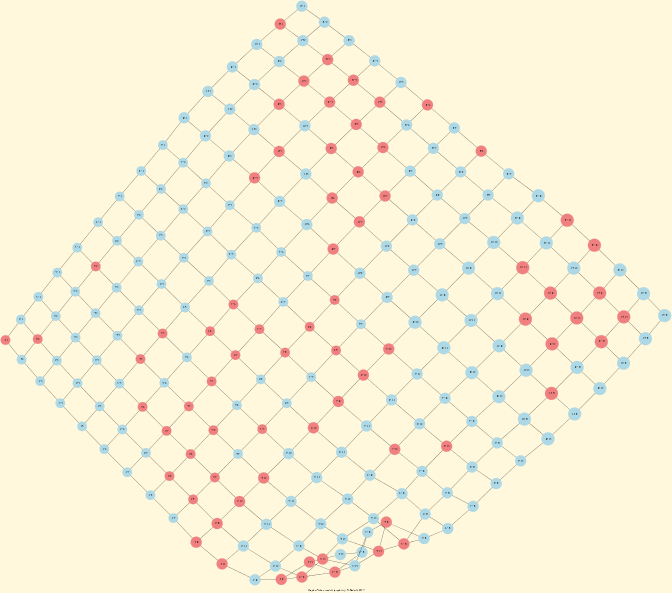
\includegraphics[width=11cm]{Figures/grid-15-15-ising.png}
\caption{Ising model of the 15x15 grid graph} 
\label{fig:22.5}       % Give a unique label
\end{figure}

\section{Simulating Metropolis random walks}
\label{sec:22.6}

Finally, we provide the \texttt{MetropolisChain} class, a specialization of the \texttt{Graph} class, for implementing a generic \emph{Metropolis} Monte Carlo Markov Chain (MCMC) sampler for simulating random walks on a given graph $g$:
\begin{lstlisting}
>>> from graphs import Graph
>>> g = Graph(numberOfVertices=5,edgeProbability=0.5)
>>> g.showShort()
  *---- short description of the graph ----*
   Name             : 'randomGraph'
   Vertices         :  ['v1', 'v2', 'v3', 'v4', 'v5']
   Valuation domain :  {'max': 1, 'med': 0, 'min': -1}
   Gamma function   :
    v1 -> ['v2', 'v3', 'v4']
    v2 -> ['v1', 'v4']
    v3 -> ['v5', 'v1']
    v4 -> ['v2', 'v5', 'v1']
    v5 -> ['v3', 'v4']
\end{lstlisting}
following a given probability $probs$ = \{‘v1’: $x$, ‘v2’: $y$, ...\} for visiting each vertex:
\begin{lstlisting}
>>> probs = {}  # initialize a potential stationary probability vector 
>>> n = g.order # for instance: probs[v_i] = n-i/Sum(1:n) for i in 1:n
>>> i = 0
>>> verticesList = [x for x in g.vertices]
>>> verticesList.sort()
>>> for v in verticesList:
...     probs[v] = (n - i)/(n*(n+1)/2)
...     i += 1
\end{lstlisting}

The \texttt{checkSampling()} method of the the \texttt{MetropolisChain} class (see below) generates a random walk of $nSim = 30000$ steps on the given graph and records by the way the observed relative frequency with which each vertex is passed by:
\begin{lstlisting}
>>> from graphs import MetropolisChain     
>>> met = MetropolisChain(g,probs)
>>> frequency = met.checkSampling(verticesList[0],nSim=30000)
>>> for v in verticesList:
...     print(v,probs[v],frequency[v])   
    v1 0.3333 0.3343
    v2 0.2666 0.2680
    v3 0.2    0.2030
    v4 0.1333 0.1311
    v5 0.0666 0.0635
\end{lstlisting}
  In this example, the stationary transition probability distribution (see Listing above), shown by the \texttt{showTransitionMatrix()} method below is quite adequately simulated.
\begin{lstlisting}
>>> met.showTransitionMatrix()
  * ---- Transition Matrix -----
    Pij  | 'v1'    'v2'    'v3'    'v4'    'v5'
    -----|-------------------------------------
    'v1' |  0.23   0.33    0.30    0.13    0.00
    'v2' |  0.42   0.42    0.00    0.17    0.00
    'v3' |  0.50   0.00    0.33    0.00    0.17
    'v4' |  0.33   0.33    0.00    0.08    0.25
    'v5' |  0.00   0.00    0.50    0.50    0.00
\end{lstlisting}

For the reader interested in algorithmic applications of Markov Chains we may recommend consulting O. Häggström's 2002 book: \citep{FMCAA}.

%%%%%%%%%
\section[The n-cycle graph]{Computing the non isomorphic MISs of the n-cycle graph}
\label{sec:22.7}

Due to the public success of our common 2008 publication with Jean-Luc Marichal \citep{ISOMIS-08} , we present in this chapter an example Python session for computing the non isomorphic maximal independent sets (MISs) from the 12-cycle graph, i.e. a \texttt{CirculantDigraph} class instance of order 12 and symmetric circulants $1$ and $-1$.
\begin{lstlisting}
>>> from digraphs import CirculantDigraph
>>> c12 = CirculantDigraph(order=12,circulants=[1,-1])
>>> c12 # 12-cycle digraph instance
  *------- Digraph instance description ------*
   Instance class   : CirculantDigraph
   Instance name    : c12
   Digraph Order    : 12
   Digraph Size     : 24
   Valuation domain : [-1.0, 1.0]
   Determinateness  : 100.000
   Attributes       : ['name', 'order', 'circulants',
                       'actions', 'valuationdomain',
                       'relation', 'gamma', 'notGamma']
\end{lstlisting}

Such $n$-cycle graphs are also provided as undirected graph instances by the \texttt{CycleGraph} class.
\begin{lstlisting}
>>> from graphs import CycleGraph
>>> cg12 = CycleGraph(order=12)
>>> cg12
  *------- Graph instance description ------*
   Instance class   : CycleGraph
   Instance name    : cycleGraph
   Graph Order      : 12
   Graph Size       : 12
   Valuation domain : [-1.0, 1.0]
   Attributes       : ['name', 'order', 'vertices',
                       'valuationDomain', 'edges',
                       'size', 'gamma']
>>> cg12.exportGraphViz('cg12')
\end{lstlisting}
\begin{figure}[h]
\sidecaption[t]
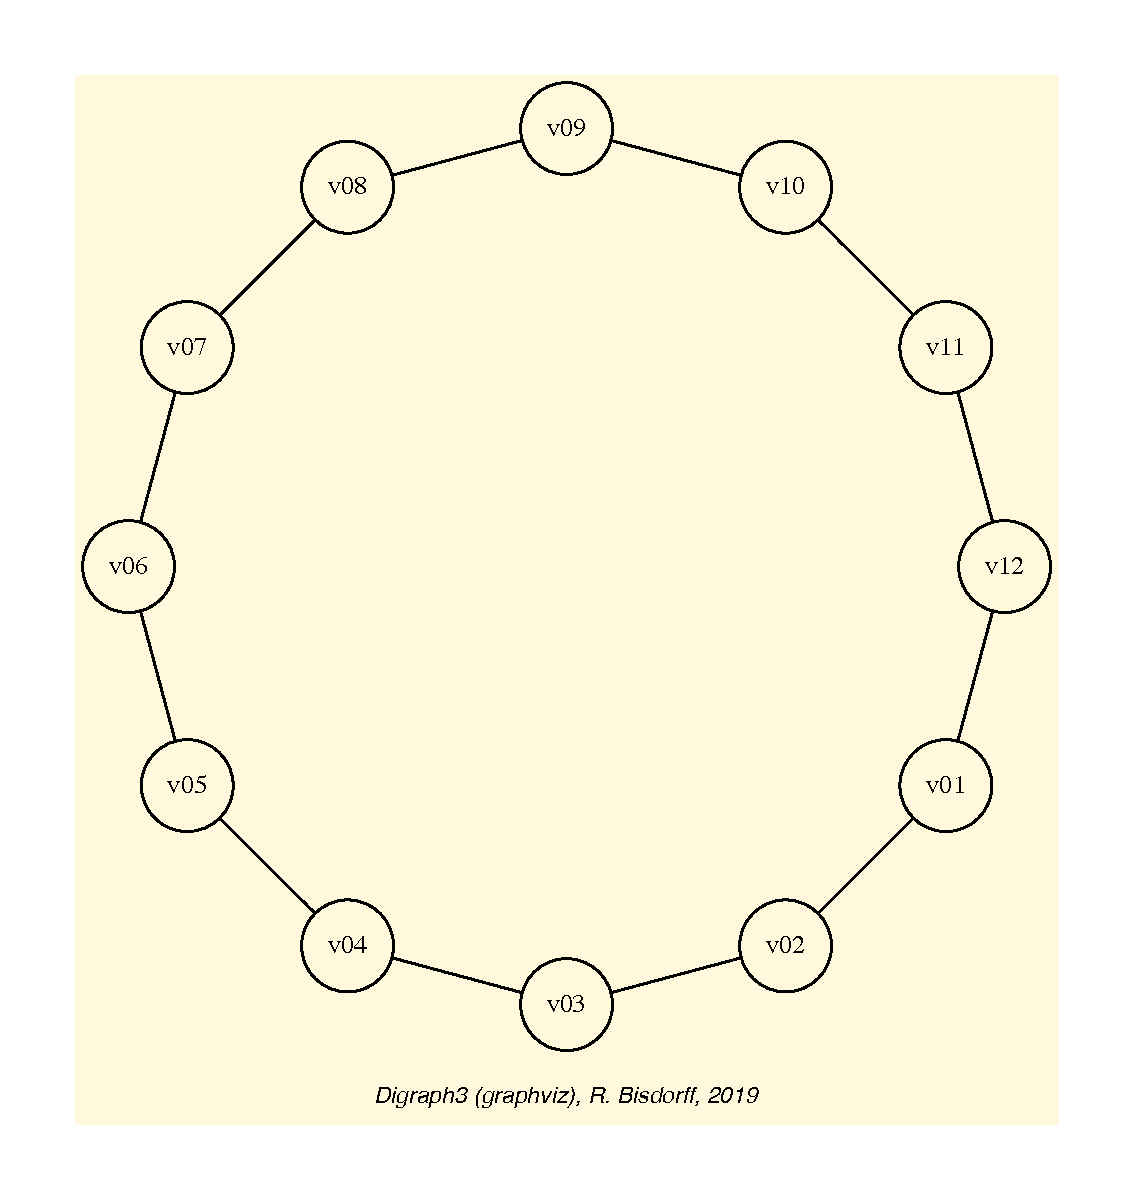
\includegraphics[width=6cm]{Figures/cg12.pdf}
\caption{The 12-cycle graph} 
\label{fig:22.7.1}       % Give a unique label
\end{figure}

\subsection{Computing maximal independent sets (MISs)}
\label{sec:22.7.1}

A non isomorphic MIS corresponds in fact to a set of isomorphic MISs, i.e. an orbit of MISs under the automorphism group of the 12-cycle graph. We are now first computing all maximal independent sets that are detectable in the 12-cycle digraph with the \texttt{showMIS()} method.
\begin{lstlisting}
>>> c12.showMIS(withListing=False)
  *---  Maximal independent choices ---*
   number of solutions:  29
   cardinality distribution
   card.:  [0, 1, 2, 3, 4,  5,  6, 7, 8, 9, 10, 11, 12]
   freq.:  [0, 0, 0, 0, 3, 24,  2, 0, 0, 0,  0,  0,  0]
   Results in c12.misset
\end{lstlisting}
In the 12-cycle graph, we observe 29 labelled MISs: 3 of cardinality 4, 24 of cardinality 5, and 2  of cardinality 6. In case of n-cycle graphs with $n$ > 20, as the cardinality of the MISs becomes big, it is preferable to use the \texttt{perrinMIS} shall command\index{perrinMIS@\texttt{perrinMIS} shell command} compiled from C and installed  along with all the \Digraph python modules for computing the set of MISs observed in the graph\footnote{The \texttt{perrinMIS} shell command may be installed system wide with the command texttt{make installPerrin} from the main \Digraph directory. It is stored by default into \texttt{/usr/local/bin/}. This may be changed with the \texttt{INSTALLDIR} flag. The command \texttt{make installPerrinUser} installs it instead without sudo into the user's private \texttt{.bin} directory.}.
\begin{lstlisting}
...$ echo 12 | /usr/local/bin/perrinMIS
  # $------------------------------------- #
  # Generating MIS set of Cn with the      #
  # Perrin sequence algorithm.             #
  # Temporary files used.                  #
  # even versus odd order optimised.       #
  # RB December 2006                       #
  # Current revision Dec 2018              #
  # -------------------------------------- #
  Input cycle order ? <-- 12
   mis 1 : 100100100100
   mis 2 : 010010010010
   mis 3 : 001001001001
    ...
    ...
    ...
   mis 27 : 001001010101
   mis 28 : 101010101010
   mis 29 : 010101010101
   Cardinalities:
   0 : 0
   1 : 0
   2 : 0
   3 : 0
   4 : 3
   5 : 24
   6 : 2
   7 : 0
   8 : 0
   9 : 0
   10 : 0
   11 : 0
   12 : 0
   Total: 29
   execution time: 0 sec. and 2 millisec.
\end{lstlisting}
Reading in the result of the \texttt{perrinMIS} shell command, stored in a file called by default \texttt{curd.dat}, may be operated with the \texttt{readPerrinMisset()} method \index{readPerrinMisset@\texttt{readPerrinMisset()}}.
\begin{lstlisting}
>>> c12.readPerrinMisset(file='curd.dat')
>>> c12.misset
    {frozenset({'5', '7', '10', '1', '3'}),
     frozenset({'9', '11', '5', '2', '7'}),
     frozenset({'7', '2', '4', '10', '12'}),
     ...
     ...
     ...
     frozenset({'8', '4', '10', '1', '6'}),
     frozenset({'11', '4', '1', '9', '6'}),
     frozenset({'8', '2', '4', '10', '12', '6'})
    }
\end{lstlisting}

\subsection{Computing the automorphism group}
\label{sec:22.7.2}

For computing the corresponding non isomorphic MISs, we actually need the automorphism group of the c12-cycle graph. The \texttt{Digraph} class therefore provides the \texttt{automorphismGenerators()} method\index{automorphismGenerators@\texttt{automorphismGenerators()}} which adds automorphism group generators to a \texttt{Digraph} class instance with the help of the external shell \texttt{dreadnaut} shell command\index{dreadnaut@\texttt{dreadnaut} shell command} from the \emph{nauty} software package \footnote{The \texttt{automorphismGenerators} method uses the \texttt{dreadnaut} shell command from the \emph{nauty} software package. See https://www3.cs.stonybrook.edu/~algorith/implement/nauty/implement.shtml . On Mac OS there exist dmg installers and on Ubuntu Linux or Debian, one may easily install it with \texttt{...\$ sudo apt-get install nauty}.}.
\begin{lstlisting}
>>> c12.automorphismGenerators()
      ...
    Permutations
    {'1':'1', '2':'12', '3':'11', '4':'10',
     '5':'9', '6':'8', '7':'7', '8':'6', '9':'5',
     '10':'4', '11':'3', '12':'2'}
    {'1':'2', '2':'1', '3':'12', '4':'11', '5':'10', 
     '6':'9', '7':'8', '8':'7', '9':'6', '10':'5', 
     '11':'4', '12':'3'}
>>> print('grpsize = ', c12.automorphismGroupSize)
   grpsize = 24
\end{lstlisting}
The 12-cycle graph automorphism group is generated with both the permutations above and has group size 24.

\subsection{Computing the isomorphic MISs}
\label{sec:22.7.3}

The \texttt{showOrbits()} method renders now the labelled representatives of each of the four orbits of isomorphic MISs observed in the 12-cycle graph (see Lines 7-10 below).
\begin{lstlisting}
>>> c12.showOrbits(c12.misset,withListing=False)
    ...
  *---- Global result ----
   Number of MIS:  29
   Number of orbits :  4
   Labelled representatives and cardinality:
   1: ['2','4','6','8','10','12'], 2
   2: ['2','5','8','11'], 3
   3: ['2','4','6','9','11'], 12
   4: ['1','4','7','9','11'], 12
   Symmetry vector
   stabilizer size: [1, 2, 3, ..., 8, 9, ..., 12, 13, ...]
   frequency      : [0, 2, 0, ..., 1, 0, ...,  1,  0, ...]
\end{lstlisting}
The corresponding group stabilizers' sizes and frequencies: orbit 1 with 6 symmetry axes, orbit 2 with 4 symmetry axes, and orbits 3 and 4 both with one symmetry axis (see Lines 12-13 above), are illustrated in the corresponding unlabelled graphs of Fig.~\ref{fig:22.7.2} below.
\begin{figure}[h]
\sidecaption[t]
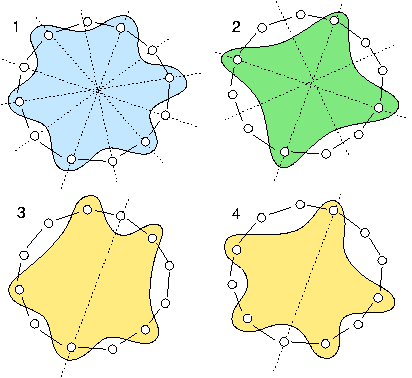
\includegraphics[width=6cm]{Figures/c12.png}
\caption{The symmetry axes of the four non isomorphic MISs of the 12-cycle graph} 
\label{fig:22.7.2}       % Give a unique label
\end{figure}

The non isomorphic MISs in the 12-cycle graph represent in fact all the ways one may write the number 12 as the circular sum of '2's and '3's without distinguishing opposite directions of writing. The first orbit corresponds to writing six times a '2'; the second orbit corresponds to writing four times a '3'. The third and fourth orbit correspond to writing two times a '3' and three times a '2'. There are two non isomorphic ways to do this latter circular sum. Either separating the '3's by one and two '2's, or by zero and three '2's (see \citep{ISOMIS-08}).


%%%%%%% The chapter bibliography
%\normallatexbib
\clearpage
%\phantomsection
%\addcontentsline{toc}{section}{Chapter Bibliography}
\bibliographystyle{spbasic}
\typeout{}
\bibliography{03-backMatters/reference}
%\chapter{Working with undirected graphs}
\label{sec:22}

\abstract*{}

\abstract{}

\section{Implementing undirected graphs}
\label{sec:22.1}

In the \Digraph {\tt graphs} module, the root \texttt{Graph} class provides a generic simple graph model, without loops and multiple links. A given object of this class contains at least the following attributes in:
\begin{enumerate}
\item \texttt{vertices}: a dictionary of vertices with \texttt{name} and \texttt{shortName} attributes,
\item \texttt{edges} : a dictionary with \emph{frozensets} \footnote{\href{https://docs.python.org/3.9/library/stdtypes.html?highlight=frozenset\#frozenset}{Python documentation}} of pairs of vertices as entries carrying a characteristic value in the range of the previous valuation domain,
\item \texttt{valuationDomain}: a dictionary with three entries: the minimum ($-1$, means certainly no link), the median ($0$, means missing information) and the maximum characteristic value ($+1$, means certainly a link),
\item \texttt{gamma}: a dictionary containing the direct neighbors of each vertex, automatically added by the object constructor.
\end{enumerate}

Example Python3 session:
\begin{lstlisting}
>>> from graphs import Graph
>>> g = Graph(numberOfVertices=7,edgeProbability=0.5)
>>> g.save(fileName='tutorialGraph')
\end{lstlisting}

The saved \texttt{Graph} instance named \texttt{tutorialGraph.py} is encoded as follows.
\begin{lstlisting}
    # Graph instance saved in Python format
    vertices = {
    'v1': {'shortName': 'v1', 'name': 'random vertex'},
    'v2': {'shortName': 'v2', 'name': 'random vertex'},
    'v3': {'shortName': 'v3', 'name': 'random vertex'},
    'v4': {'shortName': 'v4', 'name': 'random vertex'},
    'v5': {'shortName': 'v5', 'name': 'random vertex'},
    'v6': {'shortName': 'v6', 'name': 'random vertex'},
    'v7': {'shortName': 'v7', 'name': 'random vertex'},
    }
    valuationDomain = {'min':-1,'med':0,'max':1}
    edges = {
    frozenset(['v1','v2']) : -1, 
    frozenset(['v1','v3']) : -1, 
    frozenset(['v1','v4']) : -1, 
    frozenset(['v1','v5']) : 1, 
    frozenset(['v1','v6']) : -1, 
    frozenset(['v1','v7']) : -1, 
    frozenset(['v2','v3']) : 1, 
    frozenset(['v2','v4']) : 1, 
    frozenset(['v2','v5']) : -1, 
    frozenset(['v2','v6']) : 1, 
    frozenset(['v2','v7']) : -1, 
    frozenset(['v3','v4']) : -1, 
    frozenset(['v3','v5']) : -1, 
    frozenset(['v3','v6']) : -1, 
    frozenset(['v3','v7']) : -1, 
    frozenset(['v4','v5']) : 1, 
    frozenset(['v4','v6']) : -1, 
    frozenset(['v4','v7']) : 1, 
    frozenset(['v5','v6']) : 1, 
    frozenset(['v5','v7']) : -1, 
    frozenset(['v6','v7']) : -1, 
    }
\end{lstlisting}

The stored graph can be reloaded and plotted with the generic \\
\texttt{exportGraphViz()} Footnote[1] method as follows:
\begin{lstlisting}
>>> g = Graph('tutorialGraph')
>>> g.exportGraphViz()
  *---- exporting a dot file for GraphViz tools ---------*
   Exporting to tutorialGraph.dot
   fdp -Tpng tutorialGraph.dot -o tutorialGraph.png
\end{lstlisting}
\begin{figure}[h]
\sidecaption
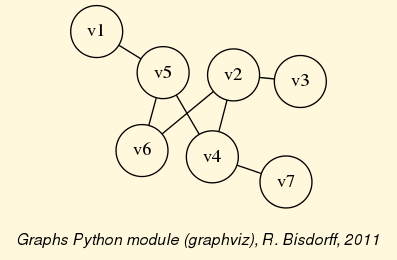
\includegraphics[width=7cm]{Figures/tutorialGraph.png}
\caption{Example simple graph instance} 
\label{fig:22.1}       % Give a unique label
\end{figure}

Properties, like the gamma function and vertex degrees and neighbourhood depths may be shown with a \texttt{showShort()} method.
\begin{lstlisting}
>>> g.showShort()
  *---- short description of the graph ----*
   Name : 'tutorialGraph'
   Vertices :  ['v1','v2','v3','v4','v5','v6','v7']
   Valuation domain : {'min': -1, 'med': 0, 'max': 1}
   Gamma function   : 
    v1 -> ['v5']
    v2 -> ['v6', 'v4', 'v3']
    v3 -> ['v2']
    v4 -> ['v5', 'v2', 'v7']
    v5 -> ['v1', 'v6', 'v4']
    v6 -> ['v2', 'v5']
    v7 -> ['v4']
   degrees      :  [0, 1, 2, 3, 4, 5, 6]
   distribution :  [0, 3, 1, 3, 0, 0, 0]
   nbh depths   :  [0, 1, 2, 3, 4, 5, 6, 'inf.']
   distribution :  [0, 0, 1, 4, 2, 0, 0, 0]
\end{lstlisting}

A \texttt{Graph} instance corresponds bijectively to a symmetric \texttt{Digraph} instance and we may easily convert from one to the other with the \texttt{graph2Digraph()}, and vice versa with the \texttt{digraph2Graph()} method. Thus, all computing resources of the \texttt{Digraph} class, suitable for symmetric digraphs, become readily available, and vice versa.
\begin{lstlisting}
>>> dg = g.graph2Digraph()
>>> dg.showRelationTable(ndigits=0,ReflexiveTerms=False)
  * ---- Relation Table -----
    S  |  'v1'  'v2'  'v3'  'v4'  'v5'  'v6'  'v7'	  
  -----|------------------------------------------
  'v1' |    -    -1    -1    -1     1    -1    -1	 
  'v2' |   -1     -     1     1    -1     1    -1	 
  'v3' |   -1     1     -    -1    -1    -1    -1	 
  'v4' |   -1     1    -1     -     1    -1     1	 
  'v5' |    1    -1    -1     1     -     1    -1	 
  'v6' |   -1     1    -1    -1     1     -    -1	 
  'v7' |   -1    -1    -1     1    -1    -1     -
>>> g1 = dg.digraph2Graph()
>>> g1.showShort()
  *---- short description of the graph ----*
   Name         : 'tutorialGraph'
   Vertices     :  ['v1','v2','v3','v4','v5','v6','v7']
   Valuation domain :   {'med': 0, 'min': -1, 'max': 1}
   Gamma function   : 
    v1 -> ['v5']
    v2 -> ['v3', 'v6', 'v4']
    v3 -> ['v2']
    v4 -> ['v5', 'v7', 'v2']
    v5 -> ['v6', 'v1', 'v4']
    v6 -> ['v5', 'v2']
    v7 -> ['v4']
   degrees      :  [0, 1, 2, 3, 4, 5, 6]
   distribution :  [0, 3, 1, 3, 0, 0, 0]
   nbh depths   :  [0, 1, 2, 3, 4, 5, 6, 'inf.']
   distribution :  [0, 0, 1, 4, 2, 0, 0, 0]
\end{lstlisting}

\section{q-coloring of a graph}
\label{25.2}

A 3-coloring of the tutorial graph $g$ may for instance be computed and plotted with the \texttt{Q\_Coloring} class as follows.
\begin{lstlisting}
>>> from graphs import Q_Coloring
>>> qc = Q_Coloring(g)
  Running a Gibbs Sampler for 42 step !
  The q-coloring with 3 colors is feasible !!
>>> qc.showConfiguration()
    v5 lightblue
    v3 gold
    v7 gold
    v2 lightblue
    v4 lightcoral
    v1 gold
    v6 lightcoral
>>> qc.exportGraphViz('tutorial-3-coloring')
  *---- exporting a dot file for GraphViz tools
   Exporting to tutorial-3-coloring.dot
   fdp -Tpng tutorial-3-coloring.dot\
                    -o tutorial-3-coloring.png
\end{lstlisting}
\begin{figure}[h]
\sidecaption
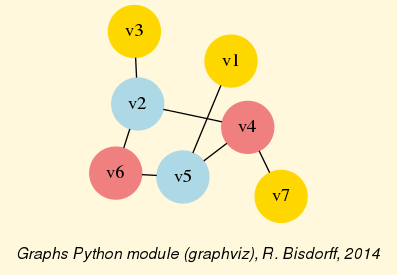
\includegraphics[width=7cm]{Figures/tutorial-3-coloring.png}
\caption{3-Coloring of the tutorial graph} 
\label{fig:22.2}       % Give a unique label
\end{figure}

Actually, with the given tutorial graph instance, a 2-coloring is already feasible.
\begin{lstlisting}
>>> qc = Q_Coloring(g,colors=['gold','coral'])
  Running a Gibbs Sampler for 42 step !
  The q-coloring with 2 colors is feasible !!
>>> qc.showConfiguration()
    v5 gold
    v3 coral
    v7 gold
    v2 gold
    v4 coral
    v1 coral
    v6 coral
>>> qc.exportGraphViz('tutorial-2-coloring')
  Exporting to tutorial-2-coloring.dot
  fdp -Tpng tutorial-2-coloring.dot\
                    -o tutorial-2-coloring.png
\end{lstlisting}
\begin{figure}[h]
\sidecaption
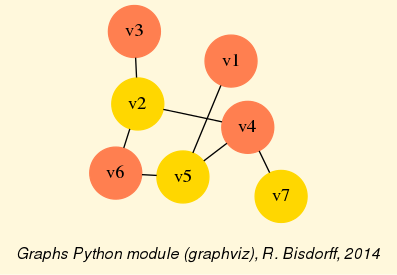
\includegraphics[width=7cm]{Figures/tutorial-2-coloring.png}
\caption{3-Coloring of the tutorial graph} 
\label{fig:22.3}       % Give a unique label
\end{figure}

\section{MIS and clique enumeration}
\label{sec:22.3}

2-colorings define independent sets of vertices that are maximal in cardinality. Computing such MISs in a given \texttt{Graph} instance may be achieved by the \texttt{showMIS} method.
\begin{lstlisting}
>>> g = Graph('tutorialGraph')
>>> g.showMIS()
  *---  Maximal Independent Sets ---*
    ['v2', 'v5', 'v7']
    ['v3', 'v5', 'v7']
    ['v1', 'v2', 'v7']
    ['v1', 'v3', 'v6', 'v7']
    ['v1', 'v3', 'v4', 'v6']
    number of solutions:  5
    cardinality distribution
    card.:  [0, 1, 2, 3, 4, 5, 6, 7]
    freq.:  [0, 0, 0, 3, 2, 0, 0, 0]
    execution time: 0.00032 sec.
    Results in self.misset
>>> g.misset
    [frozenset({'v7', 'v2', 'v5'}), 
     frozenset({'v3', 'v7', 'v5'}), 
     frozenset({'v1', 'v2', 'v7'}), 
     frozenset({'v1', 'v6', 'v7', 'v3'}), 
     frozenset({'v1', 'v6', 'v4', 'v3'})]
\end{lstlisting}

A MIS in the dual of a graph instance $g$, corresponds to a maximal \emph{clique}, i.e. a maximal complete subgraph in $g$. Maximal cliques may be directly enumerated with the \texttt{showCliques()} method.
\begin{lstlisting}
>>> g.showCliques()
  *---  Maximal Cliques ---*
    ['v2', 'v3']
    ['v4', 'v7']
    ['v2', 'v4']
    ['v4', 'v5']
    ['v1', 'v5']
    ['v2', 'v6']
    ['v5', 'v6']
   number of solutions:  7
   cardinality distribution
   card.:  [0, 1, 2, 3, 4, 5, 6, 7]
   freq.:  [0, 0, 7, 0, 0, 0, 0, 0]
   execution time: 0.00049 sec.
   Results in self.cliques
>>> g.cliques
  [frozenset({'v2', 'v3'}), frozenset({'v4', 'v7'}), 
   frozenset({'v2', 'v4'}), frozenset({'v4', 'v5'}), 
   frozenset({'v1', 'v5'}), frozenset({'v6', 'v2'}), 
   frozenset({'v6', 'v5'})]
\end{lstlisting}

\section{Line graphs and maximal matchings}
\label{sec:22.4}

The \texttt{graphs} module also provides a \texttt{LineGraph} constructor. A \emph{line graph} represents the adjacencies between edges of the given graph instance. We may compute for instance the line graph of the 5-cycle graph.
\begin{lstlisting}
>>> from graphs import CycleGraph, LineGraph
>>> g = CycleGraph(order=5)
>>> g
  *------- Graph instance description ----*
   Instance class   : CycleGraph
   Instance name    : cycleGraph
   Graph Order      : 5
   Graph Size       : 5
   Valuation domain : [-1.00; 1.00]
   Attributes       : ['name', 'order',
             'vertices', 'valuationDomain',
             'edges', 'size', 'gamma']
>>> lg = LineGraph(g)
>>> lg
  *------- Graph instance description ------*
   Instance class   : LineGraph
   Instance name    : line-cycleGraph
   Graph Order      : 5
   Graph Size       : 5
   Valuation domain : [-1.00; 1.00]
   Attributes       : ['name', 'graph',
              'valuationDomain', 'vertices',
               'order', 'edges', 'size', 'gamma']
>>> lg.showShort()
  *---- short description of the graph ----*
   Name             : 'line-cycleGraph'
   Vertices         :  [frozenset({'v1', 'v2'}),
        frozenset({'v1', 'v5'}), frozenset({'v2', 'v3'}),
        frozenset({'v3', 'v4'}), frozenset({'v4', 'v5'})]
   Valuation domain :  {'min': Decimal('-1'),
                'med': Decimal('0'), 'max': Decimal('1')}
   Gamma function   : 
    frozenset({'v1', 'v2'}) ->
         [frozenset({'v2', 'v3'}), frozenset({'v1', 'v5'})]
    frozenset({'v1', 'v5'}) ->
         [frozenset({'v1', 'v2'}), frozenset({'v4', 'v5'})]
    frozenset({'v2', 'v3'}) ->
         [frozenset({'v1', 'v2'}), frozenset({'v3', 'v4'})]
    frozenset({'v3', 'v4'}) ->
         [frozenset({'v2', 'v3'}), frozenset({'v4', 'v5'})]
    frozenset({'v4', 'v5'}) ->
         [frozenset({'v4', 'v3'}), frozenset({'v1', 'v5'})]
   degrees      :  [0, 1, 2, 3, 4]
   distribution :  [0, 0, 5, 0, 0]
   nbh depths   :  [0, 1, 2, 3, 4, 'inf.']
   distribution :  [0, 0, 5, 0, 0, 0]
\end{lstlisting}

Iterated line graph constructions are usually expanding, except for chordless cycles, where the same cycle is repeated, and for non-closed paths, where iterated line graphs progressively reduce one by one the number of vertices and edges and become eventually an empty graph.

Notice that the MISs in the line graph provide \emph{maximal matchings} --maximal sets of independent edges-- of the original graph.
\begin{lstlisting}[basicstyle=\scriptsize]
>>> c8 = CycleGraph(order=8)
>>> lc8 = LineGraph(c8)
>>> lc8.showMIS()
  *---  Maximal Independent Sets ---*
    [frozenset({'v3', 'v4'}), frozenset({'v5', 'v6'}), frozenset({'v1', 'v8'})]
    [frozenset({'v2', 'v3'}), frozenset({'v5', 'v6'}), frozenset({'v1', 'v8'})]
    [frozenset({'v8', 'v7'}), frozenset({'v2', 'v3'}), frozenset({'v5', 'v6'})]
    [frozenset({'v8', 'v7'}), frozenset({'v2', 'v3'}), frozenset({'v4', 'v5'})]
    [frozenset({'v7', 'v6'}), frozenset({'v3', 'v4'}), frozenset({'v1', 'v8'})]
    [frozenset({'v2', 'v1'}), frozenset({'v8', 'v7'}), frozenset({'v4', 'v5'})]
    [frozenset({'v2', 'v1'}), frozenset({'v7', 'v6'}), frozenset({'v4', 'v5'})]
    [frozenset({'v2', 'v1'}), frozenset({'v7', 'v6'}), frozenset({'v3', 'v4'})]
    [frozenset({'v7', 'v6'}), frozenset({'v2', 'v3'}), frozenset({'v1', 'v8'}),
     frozenset({'v4', 'v5'})]
    [frozenset({'v2', 'v1'}), frozenset({'v8', 'v7'}), frozenset({'v3', 'v4'}),
     frozenset({'v5', 'v6'})]
    number of solutions:  10
    cardinality distribution
    card.:  [0, 1, 2, 3, 4, 5, 6, 7, 8]
    freq.:  [0, 0, 0, 8, 2, 0, 0, 0, 0]
    execution time: 0.00029 sec.
\end{lstlisting}
The two last MISs of cardinality 4 (see Lines 13-16 above) give isomorphic perfect maximum matchings of the 8-cycle graph. Every vertex of the cycle is adjacent to a matching edge. Odd cycle graphs do not admit any perfect matching.
\begin{lstlisting}
>>> maxMatching = c8.computeMaximumMatching()
>>> c8.exportGraphViz(fileName='maxMatchingcycleGraph',\
...   		      matching=maxMatching)
  *---- exporting a dot file for GraphViz tools -----*
   Exporting to maxMatchingcyleGraph.dot
   Matching:  {frozenset({'v1', 'v2'}),
               frozenset({'v5', 'v6'}),
               frozenset({'v3', 'v4'}),
               frozenset({'v7', 'v8'}) }
   circo -Tpng maxMatchingcyleGraph.dot\
                  -o maxMatchingcyleGraph.png
\end{lstlisting}
\begin{figure}[h]
\sidecaption
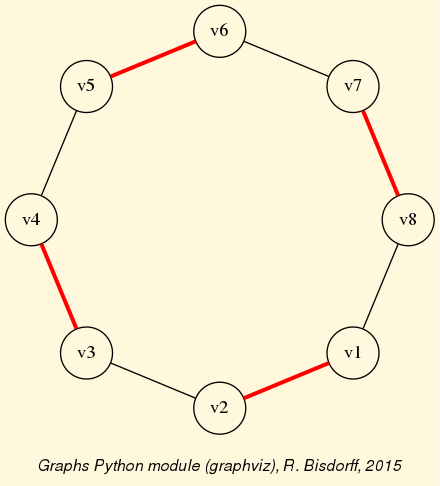
\includegraphics[width=7cm]{Figures/maxMatchingcycleGraph.png}
\caption{A perfect maximum matching of the 8-cycle graph} 
\label{fig:22.4}       % Give a unique label
\end{figure}
	    
\section{Grids and the Ising model}
\label{sec:22.5}

Special classes of graphs, like $n \times m$ rectangular or triangular grids (\texttt{GridGraph} and \texttt{IsingModel}) are available from the \texttt{graphs} module. For instance, we may use a \emph{Gibbs} sampler again for simulating an \emph{Ising Model} on such a grid.
\begin{lstlisting}
>>> from graphs import GridGraph, IsingModel
>>> g = GridGraph(n=15,m=15)
>>> g.showShort()
  *----- show short --------------*
   Grid graph    :  grid-6-6
   n             :  6
   m             :  6
   order         :  36
>>> im = IsingModel(g,beta=0.3,nSim=100000,Debug=False)
  Running a Gibbs Sampler for 100000 step !
>>> im.exportGraphViz(colors=['lightblue','lightcoral'])
  *---- exporting a dot file for GraphViz tools ---------*
   Exporting to grid-15-15-ising.dot
   fdp -Tpng grid-15-15-ising.dot -o grid-15-15-ising.png
\end{lstlisting}
\begin{figure}[h]
\sidecaption
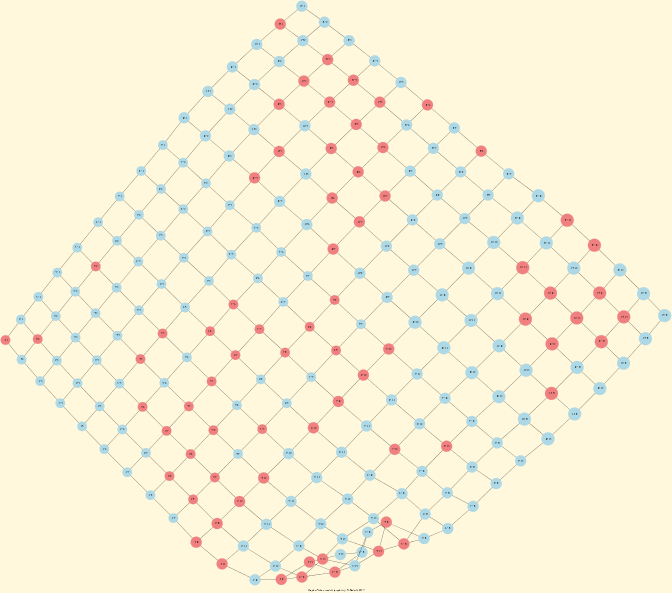
\includegraphics[width=11cm]{Figures/grid-15-15-ising.png}
\caption{Ising model of the 15x15 grid graph} 
\label{fig:22.5}       % Give a unique label
\end{figure}

\section{Simulating Metropolis random walks}
\label{sec:22.6}

Finally, we provide the \texttt{MetropolisChain} class, a specialization of the \texttt{Graph} class, for implementing a generic \emph{Metropolis} Monte Carlo Markov Chain (MCMC) sampler for simulating random walks on a given graph $g$:
\begin{lstlisting}
>>> from graphs import Graph
>>> g = Graph(numberOfVertices=5,edgeProbability=0.5)
>>> g.showShort()
  *---- short description of the graph ----*
   Name             : 'randomGraph'
   Vertices         :  ['v1', 'v2', 'v3', 'v4', 'v5']
   Valuation domain :  {'max': 1, 'med': 0, 'min': -1}
   Gamma function   :
    v1 -> ['v2', 'v3', 'v4']
    v2 -> ['v1', 'v4']
    v3 -> ['v5', 'v1']
    v4 -> ['v2', 'v5', 'v1']
    v5 -> ['v3', 'v4']
\end{lstlisting}
following a given probability $probs$ = \{‘v1’: $x$, ‘v2’: $y$, ...\} for visiting each vertex:
\begin{lstlisting}
>>> probs = {}  # initialize a potential stationary probability vector 
>>> n = g.order # for instance: probs[v_i] = n-i/Sum(1:n) for i in 1:n
>>> i = 0
>>> verticesList = [x for x in g.vertices]
>>> verticesList.sort()
>>> for v in verticesList:
...     probs[v] = (n - i)/(n*(n+1)/2)
...     i += 1
\end{lstlisting}

The \texttt{checkSampling()} method of the the \texttt{MetropolisChain} class (see below) generates a random walk of $nSim = 30000$ steps on the given graph and records by the way the observed relative frequency with which each vertex is passed by:
\begin{lstlisting}
>>> from graphs import MetropolisChain     
>>> met = MetropolisChain(g,probs)
>>> frequency = met.checkSampling(verticesList[0],nSim=30000)
>>> for v in verticesList:
...     print(v,probs[v],frequency[v])   
    v1 0.3333 0.3343
    v2 0.2666 0.2680
    v3 0.2    0.2030
    v4 0.1333 0.1311
    v5 0.0666 0.0635
\end{lstlisting}
  In this example, the stationary transition probability distribution (see Listing above), shown by the \texttt{showTransitionMatrix()} method below is quite adequately simulated.
\begin{lstlisting}
>>> met.showTransitionMatrix()
  * ---- Transition Matrix -----
    Pij  | 'v1'    'v2'    'v3'    'v4'    'v5'
    -----|-------------------------------------
    'v1' |  0.23   0.33    0.30    0.13    0.00
    'v2' |  0.42   0.42    0.00    0.17    0.00
    'v3' |  0.50   0.00    0.33    0.00    0.17
    'v4' |  0.33   0.33    0.00    0.08    0.25
    'v5' |  0.00   0.00    0.50    0.50    0.00
\end{lstlisting}

For the reader interested in algorithmic applications of Markov Chains we may recommend consulting O. Häggström's 2002 book: \citep{FMCAA}.

%%%%%%%%%
\section[The n-cycle graph]{Computing the non isomorphic MISs of the n-cycle graph}
\label{sec:22.7}

Due to the public success of our common 2008 publication with Jean-Luc Marichal \citep{ISOMIS-08} , we present in this chapter an example Python session for computing the non isomorphic maximal independent sets (MISs) from the 12-cycle graph, i.e. a \texttt{CirculantDigraph} class instance of order 12 and symmetric circulants $1$ and $-1$.
\begin{lstlisting}
>>> from digraphs import CirculantDigraph
>>> c12 = CirculantDigraph(order=12,circulants=[1,-1])
>>> c12 # 12-cycle digraph instance
  *------- Digraph instance description ------*
   Instance class   : CirculantDigraph
   Instance name    : c12
   Digraph Order    : 12
   Digraph Size     : 24
   Valuation domain : [-1.0, 1.0]
   Determinateness  : 100.000
   Attributes       : ['name', 'order', 'circulants',
                       'actions', 'valuationdomain',
                       'relation', 'gamma', 'notGamma']
\end{lstlisting}

Such $n$-cycle graphs are also provided as undirected graph instances by the \texttt{CycleGraph} class.
\begin{lstlisting}
>>> from graphs import CycleGraph
>>> cg12 = CycleGraph(order=12)
>>> cg12
  *------- Graph instance description ------*
   Instance class   : CycleGraph
   Instance name    : cycleGraph
   Graph Order      : 12
   Graph Size       : 12
   Valuation domain : [-1.0, 1.0]
   Attributes       : ['name', 'order', 'vertices',
                       'valuationDomain', 'edges',
                       'size', 'gamma']
>>> cg12.exportGraphViz('cg12')
\end{lstlisting}
\begin{figure}[h]
\sidecaption[t]
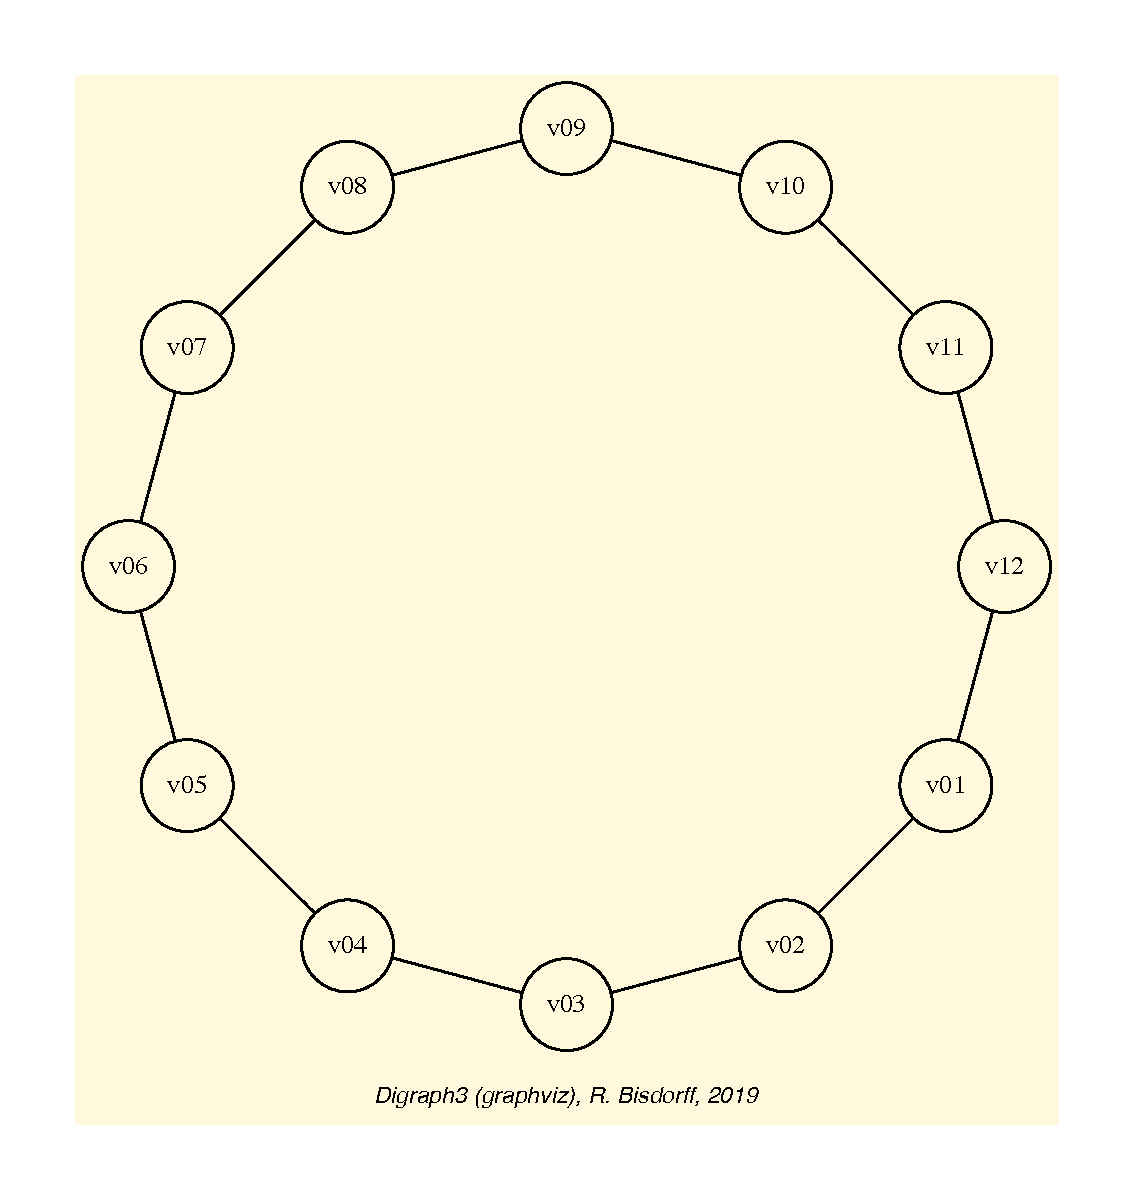
\includegraphics[width=6cm]{Figures/cg12.pdf}
\caption{The 12-cycle graph} 
\label{fig:22.7.1}       % Give a unique label
\end{figure}

\subsection{Computing maximal independent sets (MISs)}
\label{sec:22.7.1}

A non isomorphic MIS corresponds in fact to a set of isomorphic MISs, i.e. an orbit of MISs under the automorphism group of the 12-cycle graph. We are now first computing all maximal independent sets that are detectable in the 12-cycle digraph with the \texttt{showMIS()} method.
\begin{lstlisting}
>>> c12.showMIS(withListing=False)
  *---  Maximal independent choices ---*
   number of solutions:  29
   cardinality distribution
   card.:  [0, 1, 2, 3, 4,  5,  6, 7, 8, 9, 10, 11, 12]
   freq.:  [0, 0, 0, 0, 3, 24,  2, 0, 0, 0,  0,  0,  0]
   Results in c12.misset
\end{lstlisting}
In the 12-cycle graph, we observe 29 labelled MISs: 3 of cardinality 4, 24 of cardinality 5, and 2  of cardinality 6. In case of n-cycle graphs with $n$ > 20, as the cardinality of the MISs becomes big, it is preferable to use the \texttt{perrinMIS} shall command\index{perrinMIS@\texttt{perrinMIS} shell command} compiled from C and installed  along with all the \Digraph python modules for computing the set of MISs observed in the graph\footnote{The \texttt{perrinMIS} shell command may be installed system wide with the command texttt{make installPerrin} from the main \Digraph directory. It is stored by default into \texttt{/usr/local/bin/}. This may be changed with the \texttt{INSTALLDIR} flag. The command \texttt{make installPerrinUser} installs it instead without sudo into the user's private \texttt{.bin} directory.}.
\begin{lstlisting}
...$ echo 12 | /usr/local/bin/perrinMIS
  # $------------------------------------- #
  # Generating MIS set of Cn with the      #
  # Perrin sequence algorithm.             #
  # Temporary files used.                  #
  # even versus odd order optimised.       #
  # RB December 2006                       #
  # Current revision Dec 2018              #
  # -------------------------------------- #
  Input cycle order ? <-- 12
   mis 1 : 100100100100
   mis 2 : 010010010010
   mis 3 : 001001001001
    ...
    ...
    ...
   mis 27 : 001001010101
   mis 28 : 101010101010
   mis 29 : 010101010101
   Cardinalities:
   0 : 0
   1 : 0
   2 : 0
   3 : 0
   4 : 3
   5 : 24
   6 : 2
   7 : 0
   8 : 0
   9 : 0
   10 : 0
   11 : 0
   12 : 0
   Total: 29
   execution time: 0 sec. and 2 millisec.
\end{lstlisting}
Reading in the result of the \texttt{perrinMIS} shell command, stored in a file called by default \texttt{curd.dat}, may be operated with the \texttt{readPerrinMisset()} method \index{readPerrinMisset@\texttt{readPerrinMisset()}}.
\begin{lstlisting}
>>> c12.readPerrinMisset(file='curd.dat')
>>> c12.misset
    {frozenset({'5', '7', '10', '1', '3'}),
     frozenset({'9', '11', '5', '2', '7'}),
     frozenset({'7', '2', '4', '10', '12'}),
     ...
     ...
     ...
     frozenset({'8', '4', '10', '1', '6'}),
     frozenset({'11', '4', '1', '9', '6'}),
     frozenset({'8', '2', '4', '10', '12', '6'})
    }
\end{lstlisting}

\subsection{Computing the automorphism group}
\label{sec:22.7.2}

For computing the corresponding non isomorphic MISs, we actually need the automorphism group of the c12-cycle graph. The \texttt{Digraph} class therefore provides the \texttt{automorphismGenerators()} method\index{automorphismGenerators@\texttt{automorphismGenerators()}} which adds automorphism group generators to a \texttt{Digraph} class instance with the help of the external shell \texttt{dreadnaut} shell command\index{dreadnaut@\texttt{dreadnaut} shell command} from the \emph{nauty} software package \footnote{The \texttt{automorphismGenerators} method uses the \texttt{dreadnaut} shell command from the \emph{nauty} software package. See https://www3.cs.stonybrook.edu/~algorith/implement/nauty/implement.shtml . On Mac OS there exist dmg installers and on Ubuntu Linux or Debian, one may easily install it with \texttt{...\$ sudo apt-get install nauty}.}.
\begin{lstlisting}
>>> c12.automorphismGenerators()
      ...
    Permutations
    {'1':'1', '2':'12', '3':'11', '4':'10',
     '5':'9', '6':'8', '7':'7', '8':'6', '9':'5',
     '10':'4', '11':'3', '12':'2'}
    {'1':'2', '2':'1', '3':'12', '4':'11', '5':'10', 
     '6':'9', '7':'8', '8':'7', '9':'6', '10':'5', 
     '11':'4', '12':'3'}
>>> print('grpsize = ', c12.automorphismGroupSize)
   grpsize = 24
\end{lstlisting}
The 12-cycle graph automorphism group is generated with both the permutations above and has group size 24.

\subsection{Computing the isomorphic MISs}
\label{sec:22.7.3}

The \texttt{showOrbits()} method renders now the labelled representatives of each of the four orbits of isomorphic MISs observed in the 12-cycle graph (see Lines 7-10 below).
\begin{lstlisting}
>>> c12.showOrbits(c12.misset,withListing=False)
    ...
  *---- Global result ----
   Number of MIS:  29
   Number of orbits :  4
   Labelled representatives and cardinality:
   1: ['2','4','6','8','10','12'], 2
   2: ['2','5','8','11'], 3
   3: ['2','4','6','9','11'], 12
   4: ['1','4','7','9','11'], 12
   Symmetry vector
   stabilizer size: [1, 2, 3, ..., 8, 9, ..., 12, 13, ...]
   frequency      : [0, 2, 0, ..., 1, 0, ...,  1,  0, ...]
\end{lstlisting}
The corresponding group stabilizers' sizes and frequencies: orbit 1 with 6 symmetry axes, orbit 2 with 4 symmetry axes, and orbits 3 and 4 both with one symmetry axis (see Lines 12-13 above), are illustrated in the corresponding unlabelled graphs of Fig.~\ref{fig:22.7.2} below.
\begin{figure}[h]
\sidecaption[t]
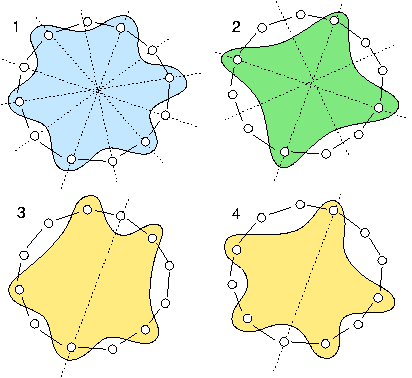
\includegraphics[width=6cm]{Figures/c12.png}
\caption{The symmetry axes of the four non isomorphic MISs of the 12-cycle graph} 
\label{fig:22.7.2}       % Give a unique label
\end{figure}

The non isomorphic MISs in the 12-cycle graph represent in fact all the ways one may write the number 12 as the circular sum of '2's and '3's without distinguishing opposite directions of writing. The first orbit corresponds to writing six times a '2'; the second orbit corresponds to writing four times a '3'. The third and fourth orbit correspond to writing two times a '3' and three times a '2'. There are two non isomorphic ways to do this latter circular sum. Either separating the '3's by one and two '2's, or by zero and three '2's (see \citep{ISOMIS-08}).


%%%%%%% The chapter bibliography
%\normallatexbib
\clearpage
%\phantomsection
%\addcontentsline{toc}{section}{Chapter Bibliography}
\bibliographystyle{spbasic}
\typeout{}
\bibliography{03-backMatters/reference}
%\input{02-mainMatters/22-chapterGraphs.bbl}